\documentclass[a4paper]{llncs}


%\documentclass[11pt]{report} % use larger type;

\usepackage[utf8]{inputenc} % set input encoding (not needed with XeLaTeX)


%%% PAGE DIMENSIONS
%\usepackage{geometry} % to change the page dimensions
\usepackage{graphicx,array}
\usepackage{amsmath}
\usepackage{amssymb}
\usepackage{amsfonts}
\usepackage{epsfig}
\usepackage{float}
%\usepackage{supertabular} % used in B Symbols
%\geometry{a4paper} % or letterpaper (US) or a5paper or....

\usepackage[english]{babel} %\usepackage{supertabular} % used in B Symbols
%\usepackage{hyperref} % add URL in bibliography
\usepackage{url} % allow add URL in document


%% Keywords for the B method

\newcommand{\MACHINE}{\ensuremath{\textbf{MACHINE }}}

%\newcommand{\MACHINE}{\operatorname{\textbf{MACHINE }}} % COMANDO ORIGINAL
\newcommand{\REFINEMENT}{\operatorname{\mathbf{REFINEMENT }}}
\newcommand{\IMPLEMENTATION}{\ensuremath{\textbf{IMPLEMENTATION }}}
\newcommand{\REFINES}{\ensuremath{\textbf{REFINES }}}
\newcommand{\SEES}{\ensuremath{\textbf{SEES }}}
\newcommand{\INCLUDES}{\ensuremath{\textbf{INCLUDES }}}
\newcommand{\IMPORTS}{\ensuremath{\textbf{IMPORTS }}}
\newcommand{\SETS}{\ensuremath{\textbf{SETS }}}
\newcommand{\CONSTANTS}{\ensuremath{\textbf{CONSTANTS }}}
\newcommand{\PROPERTIES}{\ensuremath{\textbf{PROPERTIES }}}
\newcommand{\CONCRETE}{\ensuremath{\textbf{CONCRETE }}}
\newcommand{\VARIABLES}{\ensuremath{\textbf{VARIABLES }}}
\newcommand{\ASSERTIONS}{\ensuremath{\textbf{ASSERTIONS }}}
\newcommand{\CONCRETEVARIABLES}{\ensuremath{\textbf{CONCRETE\_VARIABLES }}}
\newcommand{\DEFINITIONS}{\ensuremath{\textbf{DEFINITIONS }}}
\newcommand{\VAR}{\ensuremath{\textbf{VAR }}}
\newcommand{\IN}{\ensuremath{\textbf{IN }}}
\newcommand{\INVARIANT}{\ensuremath{\textbf{INVARIANT }}}
\newcommand{\INITIALISATION}{\ensuremath{\textbf{INITIALISATION }}}
\newcommand{\OPERATIONS}{\ensuremath{\textbf{OPERATIONS }}}
\newcommand{\BEGIN}{\ensuremath{\textbf{BEGIN }}}
\newcommand{\END}{\ensuremath{\textbf{END }}}
\newcommand{\PRE}{\ensuremath{\textbf{PRE }}}
\newcommand{\IF}{\ensuremath{\textbf{IF }}}
\newcommand{\THEN}{\ensuremath{\textbf{THEN }}}
\newcommand{\ELSE}{\ensuremath{\textbf{ELSE }}}
\newcommand{\ELSIF}{\ensuremath{\textbf{ELSIF }}}
\newcommand{\ANY}{\ensuremath{\textbf{ANY }}}
\newcommand{\WHERE}{\ensuremath{\textbf{WHERE }}}
\newcommand{\CASE}{\ensuremath{\textbf{CASE }}}
\newcommand{\OF}{\ensuremath{\textbf{OF }}}
\newcommand{\EITHER}{\ensuremath{\textbf{EITHER }}}
\newcommand{\AND}{\ensuremath{\textbf{AND }}}
\newcommand{\OR}{\ensuremath{\textbf{OR }}}
\newcommand{\NOT}{\ensuremath{\textbf{NOT }}}
\newcommand{\WHILE}{\ensuremath{\textbf{WHILE }}}
\newcommand{\DO}{\ensuremath{\textbf{DO }}}
\newcommand{\VARIANT}{\ensuremath{\textbf{VARIANT }}}
\newcommand{\FALSE}{\ensuremath{\textbf{FALSE }}}
\newcommand{\TRUE}{\ensuremath{\textbf{TRUE }}}

%% Commonly used math entities
\newcommand{\pow}{\ensuremath{\textbb{P }}}
\newcommand{\nat}{\ensuremath{\textbb{N }}}
\newcommand{\pfun}{\ensuremath{\rightarrow\mkern-22mu+}}
\newcommand{\fset}{\ensuremath{\textbb{F }}}
\newcommand{\dom}{\ensuremath{\mbox{dom}}}
\newcommand{\ran}{\ensuremath{\mbox{ran}}}
\newcommand{\natone}{\ensuremath{\textbb{N}_1}}
\newcommand{\integer}{\ensuremath{\textbb{Z }}}
%\newcommand{\fun}{\ensuremath{\rightarrow}}
\newcommand{\domr}{\ensuremath{\triangleleft}}
\newcommand{\seq}{\ensuremath{\textbf{seq1 }}}
\newcommand{\ovr}{\ensuremath{\oplus}}
\newcommand{\BOOL}{\ensuremath{\textbf{BOOL }}}
\newcommand{\pred}{\ensuremath{\textbf{pred }}}
\newcommand{\Bsucc}{\ensuremath{\textbf{succ }}}


%\usepackage{supertabular}

% DEFINITION DES CARACTERES MATHEMATIQUES B
%------------------------------------------
\def\@setmcodes#1#2#3{{\count0=#1 \count1=#3
	\loop \global\mathcode\count0=\count1 \ifnum \count0<#2
	\advance\count0 by1 \advance\count1 by1 \repeat}}

%\@setmcodes{`A}{`Z}{"7441}
%\@setmcodes{`a}{`z}{"7461}

\mathcode`\;="8000 % Makes ; active in math mode
{\catcode`\;=\active \gdef;{\semicolon\;}}
\mathchardef\semicolon="003B
%    Nominal distance from top of paper to top of page
% \topmargin 0 pt
% \textheight 53\baselineskip
% 
% %   Left margin on odd-numbered pages
% \oddsidemargin  0.15 in
% %   Left margin on even-numbered pages
% \evensidemargin 0.35 in
% %   Width of marginal notes.
% \marginparwidth 1 in
% %   Note that \oddsidemargin = \evensidemargin
% \oddsidemargin 0.25 in
% \evensidemargin 0.25 in
% \marginparwidth 0.75 in
% \textwidth 5.875 in % Width of text line.
% 
% \setlength{\parindent}{0pt}
% \setlength{\parskip}{0ex}

% DEFINITION DES FONTS
%---------------------
% The AMS extra symbol fonts are loaded.
% Note: sometimes called euxm10
\font\msx=msam10
% Note: sometimes called euym10
\font\msy=msbm10

\newfam\msxfam \textfont\msxfam=\msx
\newfam\msyfam \textfont\msyfam=\msy

\def\famletter#1{\ifcase #1 0\or 1\or 2\or 3\or 4\or 5\or 6\or 7\or
	8\or 9\or A\or B\or C\or D\or E\or F\fi}

\edef\fx{\famletter\msxfam}
\edef\fy{\famletter\msyfam}

\def\bbold{\fam\msyfam \msy}

% SYMBOLES B
%-----------
% makes a quoted expression in mathematical text
\def\token#1{\hbox{`$#1$'}}
% used for error messages in Z specs
\def\report#1{\hbox{`{\tt #1}'}}

% \@myop makes an operator, with a strut to defeat TeX's vertical adjustment.
\def\@myop#1{\mathop{\mathstrut{#1}}\nolimits}

% This underscore doesn't have the little kern --- you get an italic
% correction anyway in math mode.
\def\_{\leavevmode \vbox{\hrule width0.5em}}

% Save \q as \xq for quantifiers q.
\let\xforall=\forall
\let\xexists=\exists
\let\xlambda=\lambda
\let\xmu=\mu

% \p and \f make arrows with 1 and 2 crossings resp.
\def\p#1{\mathrel{\ooalign{\hfil$\mapstochar\mkern 5mu$\hfil\cr$#1$}}}
\def\f#1{\mathrel{\ooalign{\hfil
	$\mapstochar\mkern 3mu\mapstochar\mkern 5mu$\hfil\cr$#1$}}}

\let\mc=\mathchardef

\def	\pow		{\mbox{${\cal P}$}}
\def	\po1		{\mbox{${\cal P}_1$}}
\let	\cross		\times
\def	\lambda		{\@myop{\xlambda}}
\def	\lnot		{\neg\;}
\def	\land		{\mathrel{\wedge}}
\def	\lor		{\mathrel{\vee}}
\let	\implies	\Rightarrow
\let	\iff		\Leftrightarrow
\def	\forall		{\@myop{\xforall}}
\def	\exists		{\@myop{\xexists}}
\def	\semi		{\mathrel{\comp}}
\def	\ssemi		{\mathbin{\rm ;}}
\let	\ensembleVide	\emptyset
\let	\rel		\leftrightarrow
%\def	\dom		{\@myop{\sf dom}}
%\def	\ran		{\@myop{\sf ran}}
\def	\id		{\@myop{\sf id}}
\def	\comp		{\mathbin{\raise
			0.6ex\hbox{\oalign{\hfil$\scriptscriptstyle
			\rm o$\hfil\cr\hfil$\scriptscriptstyle\rm 9$\hfil}}}}
\def	\para		{\mbox{$\mid\mid$}}
\mc	\dres		"2\fx43
\mc	\rres		"2\fx42
\def	\ndres		{\mathbin{{\dres} \llap{$-$}}}
\def	\nrres		{\mathbin{{\rres}\llap{$-$}}}
\def	\lover		{\vartriangleleft{ \llap{$-\!\!\!\!-\!$}}}
\def	\rover		{\mathbin{{\rres}\llap{$\!-\!\!\!-$}}}
\let	\fun		\rightarrow
\def	\pfun		{\p\fun}
\def	\pinj		{\p\inj}
\mc	\inj		"3\fx1A
\def	\psurj		{\p\surj}
\mc	\surj		"3\fx10
\def	\bij		{\surj\!\!\!\!\!\!\!\inj}
\def	\nat		{\mbox{${\cal N}$}}
\def	\na1		{\mbox{${\cal N}_1$}}
\def	\num		{\mbox{${\cal Z}$}}
\def	\int		{\mbox{${\cal Z}$}}
\def	\rat		{\mbox{${\cal Q}$}}
\def	\div		{\mathbin{\rm /}}
\def	\mod		{\textbf{mod}}
\def	\upto		{\mathbin{\ldotp\ldotp}}
\def	\finset		{\mbox{${\cal F}$}}
\def	\finse1		{\mbox{${\cal F}_1$}}
\def	\ffun		{\f\fun}
\def	\finj		{\f\inj}
\def	\seq		{\@myop{\rm seq}}
\def	\cat		{\mathbin{\raise 0.8ex\hbox{$\mathchar"2\fx61$}}}
\def	\sep		{\hspace*{.05in}}

%\setcounter{secnumdepth}{0}
%\setcounter{tocdepth}{0}

%-------------------%
% Debut du document %
%-------------------%



 

%TODO: Verificar possíveis diferenças do FORMATO LNCS

% Allow use multiples footnote references 
\newcommand{\footnoteremember}[2]{
  \footnote{#2}
  \newcounter{#1}
  \setcounter{#1}{\value{footnote}}
}
\newcommand{\footnoterecall}[1]{
  \footnotemark[\value{#1}]
}


%
\begin{document}

\title{Experience in Modeling a Microcontroller Instruction Set Using B}
%
\hyphenation{se-pa-ra-te}
\hyphenation{in-struc-tion}
\hyphenation{re-gis-ter}
\hyphenation{re-gis-ters}

%
%
%
\author{Val\'{e}rio Medeiros Jr\inst{1}, David D\'{e}harbe\inst{2}}


\institute{Federal Institute of Education, Science and Technology of Rio Grande do Norte, Natal, RN, Brazil
  \and 
  Federal University of Rio Grande do Norte, Natal, RN, Brazil}

\maketitle


\begin{abstract}

  This paper presents a formal model, developed in B, of the Z80
  instruction set. The formal model includes different libraries that
  specify entities commonly used in microcontrolers and
  microprocessors. Not only this model can be used for documentation
  purposes, but also to simulate and test the assembly code. It is also
  a fundamental component to extend the reach of the B method from the
  specification of the functional requirements of a system to an assembly-level
  implementation thereof.
% Using this model-driven approach and the instruction set model, a small case
% study to analyse a petroleum production test system in oil field was developed.
%  \paragraph[Keywords]{ \textbf{Keywords}: Embedded Software, Simulation, B
% method and Verification%}
\end{abstract}



\section{Introduction}

The B method~\cite{Abrial} supports the formal development of software
from a specification of functional requirements down to an imperative
implementation of those requirements, amenable to synthesis to a
programming language such as C or Ada. However, the synthesis step is
not amenable to proof of correctness, and~\cite{Dantas_SBMF08} proposed
an approach to extend the scope of the B method up to the assembly
level language. One key component of this approach is to build, within
the framework of the B method, formal models of the instruction set of
such assembly languages.

This work presents a formal model of the instruction set of the Z80
microcontroller~\cite{Z80_manual}. This microcontroller was chosen
because of several factors: it contains essential and common concepts
of microcontrollers and even microprocessors; it has extensive
available documentation; and it has been widely used.  A first,
partial, Z80 model presented in \cite{Valerio_SBMF09} was fully
verified, but it used constructs that made it impossible to animate.

The new model supports animation in ProB~\cite{proB}.  Essentially, the
new model\footnote{The interested reader in more details is invited to
  visit our repository at: http://code.google.com/p/b2asm/.}  no
longer contains definitions derived from infinite sets. Using B
constructs for modularity, auxiliary libraries of basic modules were
developed as part of the construction of the microcontroller model. Such
a library has many definitions of concepts common to microcontrollers.
Besides the new Z80 model, a petroleum production test system was
developed using the Z80 assembly language to analyse the code simulation
and the verification process.

The formal model of an instruction set has several
applications. Animation allows to simulate the execution of assembly
programs including support for interrupts, input and output
instructions. Other possible uses include documentation, the
construction of simulators, and can possibly be the starting point of
a verification effort for the actual implementation of a Z80
design. Moreover, the model of the instruction set could be
instrumented with non-functional aspects, such as the number of cycles
it takes to execute an instruction, to prove lower and upper bounds on
the execution time of a routine.  Two aspects of such formalizations
are of particular importance to us: provide a more solid documentation
artifact for microcontrollers and build a reference model for a formal
compilation approach in B.

It is often the case that the official documentation of an instruction
uses textual description, mathematical formulas, examples,
etc. Sometimes, the instruction descriptions have a specific notation,
some informations are organized in different sections of a document and
the textual descriptions are not standardized.  The manuals also have
semi-formal and informal descriptions, these descriptions may leave
errors, inconsistency and ambiguity.  For example, in the official
manual of the microcontroller Z80 \cite{Z80_manual}, the semantics of
an instruction (in particular its effects on the flag register) are
described informally, and this description is scattered in
different pages.  Furthermore, the official manual of the
microcontroller Z80 has also several problems that were identified
over time~\cite{UndocumentedZ80}.

A solution to avoid ambiguity and inconsistencies is to formally
specify the assembly instruction set, making it possible to prove
properties of the instructions. The formal model also restricts the
definitions to correct typing and uses only well-defined
expressions. Furthermore, the developer may use the refinement
capabilities of the B method to specify at different levels of
abstraction and add more specific details or useful restrictions in
refined models.

%In general, the manuals of microcontrollers can be more suited for
%developers in assembly language. Many times, each instruction of microcontrollers
%is shown in its official manual using textual description, math description, examples,
%encoding, number of cycles and other information.Some times, the instruction descriptions
%have an own notation, some informations are organized in different sections of document 
%and the textual description are not standardized. This does not allow the interpretation by parser.
%% b) The case of Z80
%For example in official manual of the microcontroller Z80 \cite{Z80_manual}, if the users
%want to know the action of an instruction and its effects on the flag register then he needs
%to read an informal textual description. So, this description can add
%some ambiguities or even mistakes. The official manual has also several problems that were 
%identified over time~\cite{UndocumentedZ80}. The Z80 is a microcontroller that  has been
%tested and used for many years. This intensive use and test facilitated to find several
%errors in the description of the instructions in its manual. Several of these problems
%have been reported in a technical report \cite{UndocumentedZ80}. Some problems are inaccurate
%information, for example the description of the action of an instruction on the flag
%register, partial information and distributed on different pages of manual.
%
%
%% in the Z80 manual happens was that,
%
%%A simple example of error is in some official documentation saying that a group of instructions leaves the \textit{CF} flag unaffected and the \textit{NF}
%%flag is not always set, but may also be reset \cite{UndocumentedZ80}.
%%% \begin{itemize} \item Some input and output instructionsThe
%%% INI/INIR/IND/INDR/OUTI/OUTD/OTIR/OTDR instructions do affect the CF flag (some
%%% official documentation says they leave it unaffected, important!) and the NF
%%% flag is not always set but may also be reset (see 4.3 for exact operation)
%%% \cite{UndocumentedZ80}. Este erro he descrito na phegina (274 do documento e
%%% 294 do pdf) do manual oficial do Z80 (Z80_CPU_adotado.pdf) Citar apenas esse
%%% exemplo abaixo! \item
%%%when a determined interruption (NMI) is accepted, the bit IFF1 is not   
%%%copied to bit IFF2~\cite{UndocumentedZ80}. 
%%%
%%This example can cause serious problems for programmers.
%%% Este erro he descrito na pagina (22 do documento e 26do pdf) do manual
%%% official do Z80 (Z80_CPU_adotado.pdf) Only IFF1 is reset.
%%This error and others 7 different errors were previously identified by~\cite{UndocumentedZ80}. So to help the 
%%construction of Z80 B model, other references~\cite{UndocumentedZ80,Simulator_z80}
%%were also consulted.
%
%A solution to avoid ambiguity and inconsistencies is to specify formally the
%assembly instruction set, this creates a pattern of representation and validates
%properties of instructions. The formal model also restricts the definitions to
%correct typing and uses only well-defined expressions. Furthermore, the developer
%can use with B method different levels of abstraction and add more specific details
%in refined models.
% 
%Finally, the main goal of this project, though, is to provide a basis for the
%generation of software artefacts at the assembly level, those are amenable to 
%refinement verification within the B method.

%\subparagraph{Report structure}
%
%This work is focused on the presentation of modelling of assembly instruction
%set, including elementary libraries to describe hardware aspects; and the
%modelling and simulation of a case study of an embedded verified software that
%can be used in tanks of the petroleum industry.   

This paper is structured as follows.  Section~\ref{sec:models}
presents the elementary libraries and the modeling of some elements
common to microcontrollers.  Section~\ref{sec:z80} presents the B
model of the Z80 instruction set.  Related work are discussed in
section~\ref{sec:relatedworks}. Finally, the last section is devoted
to the conclusions.

%
%\section{Introduction to the B Method}
%\label{sec:B_method}
%
%The B method for software development~\cite{Abrial} is based on the B Abstract
%Machine Notation (AMN) for the formal specification of functional requirements and the use of formally proved refinements up to a
%specification sufficiently concrete that programming code can be automatically
%generated from it. Its mathematical basis consists of first order logic, integer
%arithmetic and set theory, and its corresponding constructs are similar to those
%of the Z notation~\cite{Spivey96}.
%
%A B specification is structured in modules. A module defines a set of valid
%states, including a set of initial states, and operations that may provoke a
%transition among states. The design process starts with a module with a
%so-called functional model of the system under development. In this initial
%modelling stage, the B method requires that the user proves that, in a machine,
%all its initial states are valid, and operations do not define
%transitions from valid states to invalid states.
%
%
%Essentially, a B module contains two main parts: a header and the available
%operations. Figure~\ref{fig:maqB} has a very basic example. The clause
%\MACHINE  has the name of module.  The next two clauses, respectively,
%reference external modules and create an instance of an external module.  The
%\VARIABLES clause declares the name of the variables that compose the
%state of the machine. Next, the \INVARIANT clause defines the valid states,
%specifying  the type and other restrictions on the variables. The \INITIALISATION specifies
%the initial states. Finally, operations correspond to the transitions among
%states of the machine.
%
%
%\begin{figure}[h]
%  % \begin{small}
%\begin{center}
%\begin{sloppypar}
%
%  $\begin{array}{lcl}
%    \begin{array}[t]{l}
%      \MACHINE \quad  \textit{micro} \\
%      \SEES \quad \textit{TYPES}, \textit{ALU} \\
%      \INCLUDES  \quad \textit{MEMORY} \\
%      \VARIABLES \quad    \textit{pc}  \\
%      \INVARIANT\\ 
%      \quad \textit{pc} \in \textit{INSTRUCTION} 
%    \end{array}
%    & \hspace*{0cm} &
%    \begin{array}[t]{l}
%      \INITIALISATION  \textit{pc} := 0 \\
%      \OPERATIONS\\
%      \textit{JMP} \textit{( jump )} = \\
%      \quad \PRE \textit{jump} \in \textit{INSTRUCTION}\\ 
%      \quad \THEN \textit{pc} := \textit{jump}\\  
%      \quad \END \\
%      \END
%    \end{array}
%  \end{array}
%  $
% \end{sloppypar} 
%\end{center}
%\caption{A very basic B machine.}
%\label{fig:maqB}
%\end{figure}



\section{Model structure and basic components}
\label{sec:models}
%Em cada subsecaoo descrever os principais lemas que foram provados.
%Sugestheo de David:
% a) structure
% b) formalization of bit-level concepts
% c) formalization of bit vectors
% d) formalization of byte and word-level concepts
% e) formalization of integer ranges 

We have developed a reusable set of basic definitions to model
hardware concepts and data types concepts. The models contain
definitions to represent: registers, interruptions, input and
output ports, memory and instructions. These definitions are grouped
into separated development projects and are available as libraries.
Thus the workspace is composed of the following: 
\begin{description}

\item[Power] contains the standard definition of exponentiation, as
  well as some basic properties, e.g. values of different powers of
  two. Given this definition, these properties have been proved
  interactively with the Atelier-B prover.

\item[Hardware Library] defines bit vectors with size 8 and 16, basic
  functions to manipulate bit vectors and important
  assertions. Details are given in sections
  \ref{subsec:HardwareLibrary1}, \ref{subsec:HardwareLibrary2} and
  \ref{subsec:HardwareLibrary3}.
 
\item[Types Library] defines sets of naturals and integers represented
  with 8 bits and 16 bits, basic conversion functions between those
  types and bit vectors, and important assertions. It is presented in
  section \ref{subsec:Types}.
 
\item[Platform] defines functions of the arithmetic logic unit, memory
  unit, registers and assembly instructions. Section \ref{sec:z80}
  provides additional details.
 
\end{description}

The dependencies between those libraries are depicted in
Figure~\ref{fig:hardware-definition-graph}.

\begin{figure}[h]
\centering
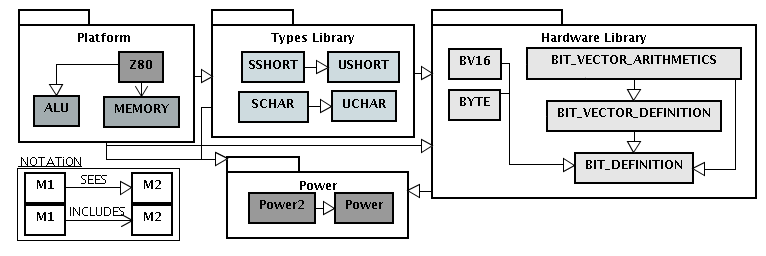
\includegraphics[width=.77\textwidth]{diagramaEstrutural_vertical_ProB.png}
 \caption{Dependency diagram of the Z80 model.}
\label{fig:hardware-definition-graph}
\end{figure}

\subsection{Bit representation and manipulation}
\label{subsec:HardwareLibrary1}

The entities defined in the module $\textit{BIT\_DEFINITION}$ are the
type for bits, logical operations on bits (negation, conjunction,
disjunction, exclusive disjunction), and a conversion function from
Booleans to bits.

We model bits as a set of integers: $\textit{BIT} =
\textit{0..1}$. The negation is an unary function on bits and it is
defined as:
$$
\begin{array}{l}
\textit{bit\_not}  \in  \textit{BIT}  \fun  \textit{BIT}  \land 
\textit{bit\_not} \rm = \rm \{ \rm 0  \mapsto  \rm 1 , \rm 1  \mapsto  \rm 0 \rm \}
\end{array}
$$
%\forall ( \textit{bb}). (\textit{bb} \in \textit{BIT} \implies {bit\_not}(\textit{bb}) =1-\textit{bb})\\

The module also provides lemmas on negation that may be useful for the
users of the library to develop proofs:
$$
\begin{array}{l}
%  \textit{bit\_not}(0) = 1;  \textit{bit\_not}(1) = 0; \\
\forall (\textit{bb}).(\textit{bb} \in \textit{BIT} \implies \textit{bit\_not}(\textit{bit\_not}(\textit{bb})) = \textit{bb})
\end{array}
$$
Conjunction is a binary function on bits and it is defined as:
$$
\begin{array}{l}
\textit{bit\_and} \in \textit{BIT} \times \textit{BIT} \fun \textit{BIT} \land \\
\forall (\textit{b1}, \textit{b2}).(\textit{b1}  \in \textit{BIT}  \land \textit{b2} \in \textit{BIT} \implies \\
\quad ((\textit{bit\_and}(\textit{b1}, \textit{b2}) = 1) \iff (\textit{b1} = 1)  \land  (\textit{b2} = 1)))
\end{array}
$$
The module provides the following lemmas for commutativity and associativity:
$$
\begin{array}{l}
%  \textit{bit\_and}(0,0) = 0;  \textit{bit\_and}(0,1) = 0; \\
%  \textit{bit\_and}(1,0) = 0;  \textit{bit\_and}(1,1) = 1; \\
\forall (\textit{b1},\textit{b2}).(\textit{b1} \in \textit{BIT} \land \textit{b2} \in \textit{BIT} \implies \\
\quad (\textit{bit\_and}(\textit{b1}, \textit{b2}) = \textit{bit\_and}(\textit{b2},\textit{b1})))\land \\
\forall (\textit{b1},\textit{b2},\textit{b3}).(\textit{b1} \in \textit{BIT} \land  \textit{b2} \in \textit{BIT} \land \textit{b3} \in \textit{BIT} \implies \\
\quad (\textit{bit\_and}(\textit{b1}, \textit{bit\_and}(\textit{b2},\textit{b3})) = \textit{bit\_and}(\textit{bit\_and}(\textit{b1},\textit{b2}),\textit{b3})))\\
% \forall (\textit{b1}).(\textit{b1} \in \textit{BIT} \implies (\textit{bit\_and}(\textit{b1}, 1) = \textit{b1})); \\
% \forall (\textit{b1}).(\textit{b1} \in \textit{BIT} \implies (\textit{bit\_and}(\textit{b1}, 0) = 0));
\end{array}
$$
The module provides definitions of $\textit{bit\_or}$ (disjunction)
and $\textit{bit\_xor}$ (exclusive disjunction), as well as lemmas on
those operators. These are standard and their expression in B is
similar to $\textit{bit\_and}$.

Finally, the conversion from Boolean to bit is simply defined as:
$$
\begin{array}{l}
\textit{bool\_to\_bit} \in \BOOL \fun \textit{BIT} \land \textit{bool\_to\_bit} = \{ \TRUE \mapsto 1, \FALSE \mapsto 0 \} \\
\end{array}
$$
All the lemmas that are provided in this module have been
automatically proved by the prover of Atelier-B.


\subsection{Representation and manipulation of bit vectors}
\label{subsec:HardwareLibrary2}

Sequences are predefined objects in B and are natural candidates to
represent bit vectors. In B, sequences are functions whose domain
is an integer range with lower bound 1 (one). Indices in bit vectors
usually range from 0 (zero) upwards and the model we propose obeys
this convention by making an offset where necessary, so that
predefined functions and proof rules may be used. We define bit
vectors as non-empty sequences of bits: $\textit{BIT\_VECTOR} =
\seq1 (\textit{BIT})$. As $\textit{BIT\_VECTOR}$ is an infinite set,
this definition hinders the animation in ProB.  As a workaround, we
defined specialized types \textit{BYTE} and \textit{BV16} without
reference to \textit{BIT\_VECTOR}.

% CAN COMMENT TO REDUCE SPACE
%The function $\textit{bv\_size}$ returns the size of a given bit vector. It is basically a wrapper for the
%predefined function $\textbf{size}$ that applies to sequences.
%
%$
%\begin{array}{l}
%\textit{bv\_size} \in \textit{BIT\_VECTOR} \fun \nat_1 \land \\
%\textit{bv\_size} = \lambda bv . (bv \in \textit{BIT\_VECTOR} \mid \textbf{size}(bv))
%\end{array}
%$

We also define two functions $\textit{bv\_set}$ and
$\textit{bv\_clear}$ that, given a bit vector, and a position in a
bit vector, returns the bit vector resulting from setting the
corresponding position to 1 and 0, and a function $\textit{bv\_get}$
that, given a bit vector and a valid position, returns the value of
the bit at that position. Only the first definition is shown here:
$$
\begin{array}{l}
\textit{bv\_set} \in \textit{BIT\_VECTOR} \times \nat \fun \textit{BIT\_VECTOR} \land \\ \textit{bv\_set} =
\lambda v, n . (v \in \textit{BIT\_VECTOR} \land n \in \nat \land n <\textit{size}(v)
\mid v \lover \{ n+1 \mapsto 1 \})
\end{array}
$$

Function $bv\_catenate$ takes as parameters two bit vectors $v$ and
$w$, and returns the concatenation of $v$ and $w$, such
that $v$ constitutes the most significant part of the result.


% $
% \begin{array}{l}
% \textit{bv\_catenate} \in \textit{BIT\_VECTOR} \times \textit{BIT\_VECTOR} \fun \textit{BIT\_VECTOR} \land \\
% \textit{bv\_catenate} = \lambda v, w \bullet (v \in \textit{ BIT\_VECTOR} \land w \in \textit{ BIT\_VECTOR}  \mid v 
% %\conc
%   w)
% \end{array}
% $


\hspace*{0.00in} \it bv\_catenate  $\in$  \it BIT\_VECTOR  $\times$  \it BIT\_VECTOR  $\fun$ \it
BIT\_VECTOR $\land$\\
\hspace*{0.21in} \it bv\_catenate \rm =  $\lambda$  v\rm ,\it w \rm . \rm (\it v 
$\in$  \it BIT\_VECTOR $\land$ \it w $\in$  \it BIT\_VECTOR  $\mid$  \it v\^ \it w\rm ) %$\cat$

%COMMENT TO REDUCE SPACE
%We also define a function $\textit{bv\_zero}$ that, given a positive
%integer $n$, return a bit vector of size $n$, with all bits set to 0.
%A similar function, called $\textit{bv\_one}$, with all bits set to 1
%is also defined but not presented here.
%
%$
%\begin{array}{l}
%\textit{bv\_zero} \in \nat_1 \fun \textit{BIT\_VECTOR} \land \\
%\textit{bv\_zero} = \lambda n . (n \in \nat_1 \mid 1..n \times \{0\}) 
%\end{array}
%$
%


Additionally, the module provides definitions for the classical
logical combinations of bit vectors: $\textit{bit\_not}$,
$\textit{bit\_and}$, $\textit{bit\_or}$ and $\textit{bit\_xor}$. Only
the first two are presented here. The domain of the binary operators
is restricted to pairs of bit vectors of the same length:
$$
\begin{array}{l}
\textit{bv\_not} \in \textit{BIT\_VECTOR} \fun \textit{BIT\_VECTOR} \land \\
\textit{bv\_not} = \lambda v . (v \in \textit{BIT\_VECTOR} \mid \quad \lambda i . (1 .. \textit{size}(v)) \mid \textit{bit\_not}(v(i))) \land \\
\textit{bv\_and} \in \textit{BIT\_VECTOR} \times \textit{BIT\_VECTOR} \fun \textit{BIT\_VECTOR} \land \\
\textit{bv\_and} = \lambda v_1, v_2 . (v_1 \in \textit{BIT\_VECTOR} \land v_2 \in \textit{BIT\_VECTOR} \land \\
\textit{size}(v_1) = \textit{size}(v_2) \mid \lambda i . (1 .. \textit{size}(v_1)) \mid
\textit{bit\_and}(v_1(i), v_2(i)))
\end{array}
$$
We provide several lemmas on bit vector operations. These lemmas
express properties on the size of the result of the operations
as well as classical algebraic properties such as associativity
and commutativity.

\subsection{Modeling bytes and bit vectors of length 16}
\label{subsec:HardwareLibrary3}

Bytes, i.e. bit vectors of length 8, are a common entity in hardware
design. We provide the following definitions:

\hspace*{0.0in}\it BYTE\_WIDTH \rm = 8 $\land$ \it BYTE\_INDEX \rm = 1 $\upto$ \rm  BYTE\_WIDTH\rm  \hspace*{0.03in} $\land$

\hspace*{0.0in}\it PHYS\_BYTE\_INDEX \rm = \rm 0 $\upto$ \rm (\it BYTE\_WIDTH\rm -\rm 1\rm )\hspace*{0.03in} $\land$ \hspace*{0.0in}\it BYTE \rm =\rm (\it BYTE\_INDEX  $\fun$  \it BIT\rm )\hspace*{0.0in} $\land$  


\hspace*{0.0in}$\forall$ \rm (\it b1\rm )\rm .\rm (\it b1  $\in$  \it BYTE  $\implies$  \bf size\rm (\it b1\rm )\rm =\it BYTE\_WIDTH  $\land$  \it b1  $\in$  \bf seq1\rm (\it BIT\rm )\rm ) 

%\hspace*{0.0in}\it BYTE \rm = \rm \{ \it bt  $\mid$  \it bt $\in$ \it BIT\_VECTOR  $\land$  \it size\rm (\it bt\rm )\rm =\it BYTE\_WIDTH\rm \} $\land$

%\hspace*{0.0in}\it BYTE\_ZERO  $\in$  \it BYTE  $\land$ \it BYTE\_ZERO \rm = \it BYTE\_INDEX  $\times$  \rm \{\rm 0\rm \}

$\textit{BYTE\_INDEX}$ is the domain of the functions modeling
bytes. It starts at 1 to be compatible with sequences. However, since
the hardware community starts indexing from zero, definition
$\textit{PHYS\_BYTE\_INDEX}$ provides functionalities obeying this
convention. Type $\textit{BYTE}$ is as a specialized type of
$\textit{BIT\_VECTOR}$, with a size constraint. Other specific
definitions are provided to facilitate further modeling: the type
$\textit{BV16}$ is created for bit vectors of length 16 in a similar
way.

\subsection{Bit vector arithmetic}
\label{subsec:Types}
 

Bit vectors are used to represent and combine numbers: integer ranges
(signed or unsigned). Therefore, our library includes functions to
manipulate such data, for example, the function $\textit{bv\_to\_nat}$
maps bit vectors to natural numbers:
$$
\begin{array}{l}
\textit{bv\_to\_nat} \in \textit{BIT\_VECTOR} \fun \nat  \land \\
\textit{bv\_to\_nat} = \lambda v .  (v \in \textit{BIT\_VECTOR} \mid  \sum i . (i \in \dom(v) . v(i)
\times 2^{i-1}))
\end{array}
$$

An important lemma associated to this definition is: 
$$\forall n . (n \in \nat_1 \implies \textit{bv\_to\_nat}(\textit{nat\_to\_bv}(n)) = n).$$



\subsection{Basic data types}

The definition of instruction sets usually have bit vector and integer
types as listed in table~\ref{tab:types}. For each type, a number of
functions are defined, including conversion between different types.

\begin{table}[h]
\caption{Details of basic data types}
\label{tab:types}
\begin{center}
\begin{tabular}{|c|c|c|c|c|}
\hline
 \textit{Type\ Name} & \textit{Range} & \textit{Physical Size}  & \textit{Num. POs} & \textit{Library} \\\hline
 BIT & 0..1 & 1 bit &   118 & Hardware \\\hline 
 BYTE & -- & 1 bytes &  154 & Hardware \\\hline
 BV16 & -- & 2 bytes &  75 & Hardware \\ \hline
 UCHAR & 0..255 & 1 byte &  30 & Types \\\hline
 SCHAR & -128..127 & 1 byte & 30 & Types \\\hline 
 USHORT & 0..65535 & 2 byte & 62 & Types \\\hline
 SSHORT & -32768..32767 & 2 bytes & 62 & Types \\\hline 
\end{tabular}
\end{center}
\end{table}

Usually, each type module just needs to specialize definitions that
are given in the hardware modeling library.  For example, the function
$\textit{bv\_to\_nat}$ from bit vector arithmetic is specialized to
$\textit{byte\_uchar}$. As the set $\textit{BYTE}$ is a subset of the
$\textit{BIT\_VECTOR}$, this function can be defined as follows:
$$
\begin{array}{l}
\textit{byte\_uchar} \in \textit{BYTE} \fun \nat \land \\
\textit{byte\_uchar} = \lambda (v) . ( v \in BYTE | bv\_to\_nat(v) )
\end{array}
$$

The definitions of the library types reuse the basic definitions from
the hardware library. This provides greater confidence and facilitates
the proof process, because the prover can reuse the previously defined
lemmas.


%The inverse function $\textit{uchar\_byte}$ is easily defined:
%
%$
%\begin{array}{l}
%\textit{uchar\_byte} \in \textit{UCHAR}  \fun  \textit{BYTE}  \land \\
%   \textit{uchar\_byte} = \ (\textit{byte\_uchar}) ^{-1}
%\end{array}
%$

We also created lemmas on pairs of dual conversion functions, such as:
$$
 \begin{array}{l}
  \forall (val) . (val \in \textit{UCHAR} |
  \textit{byte\_uchar}(\textit{uchar\_byte}(val)) = val) \land\\
  \forall (by) . (by \in \textit{BYTE} |
  \textit{uchar\_byte}(\textit{byte\_uchar}(by)) = by)
 \end{array}
$$

%TODO:[NEW PARAGRAPH-TO-REVIEW]
Similarly, several other general functions and lemmas were created for all other data types.
Some times, we need  create arithmetic and logic functions that are more specific for a
determined microprocessor, like Z80 that is presented in the section \ref{sec:z80}. 

%TODO:[NEW PARAGRAPH-TO-REVIEW]
The definitions, functions and properties from hardware library and types library are difficult to verify,
on the other hand  these libraries can be reused in several others  microprocessors without to verify again.
Nearly 50\% of all these proof obligations shown in the Table~\ref{tab:types} are verified automatically 
or with few user pass\footnote{The user pass are steps that aid the prover to find the proof.} .
But many others proof obligations are difficult to verify, because they involve functions
that contain arithmetic expressions that are complex to manipulate with the interactive
prover of AtelierB.  However, all theses 531 proof obligations were verified completely.


\subsection{Verification of hardware library and types library} 
\label{sec:VerificationHardwareLibrary}

This section presents the verification of the aforementioned modules
using AtelierB provers.  By default, AtelierB~\cite{atelierB} does not
generate proof obligations to check the type of functions defined in
the $PROPERTIES$ clause of a machine. For example, the definition $inc
\in \{0,1\} \fun \{0,1\} \land inc = \lambda(x).( x \in \{0,1\} | x +
1)$, does not create a proof obligation to check the consistency of
the definition. However, this definition is inconsistent since
$inc(1)=2$ and $ 2 \not\in \{0,1\}$.

To avoid such inconsistencies, we state separately the required
properties in the \textit{ASSERTIONS\/} clause: this causes
corresponding proof obligations to be generated and verified. However,
we have not been able to build the corresponding proofs using the 
rule base included in the free distribution of AtelierB. So we
formalized new proof rules to check these properties in AtelierB and
used them in the interactive prover of AtelierB.

The hardware library has many conversion functions with
arithmetic,  for example, Bit\_vector to Natural, Natural to
Bit\_vector, Integer to Bit\_vector and Bit\_vector to Integer. These
functions are organized in modules and each module contains auxiliary
functions for a data type. The modules are represented by gray
rectangles in Figure \ref{DiagramTypesRules}.

\begin{figure}[he]
\centering
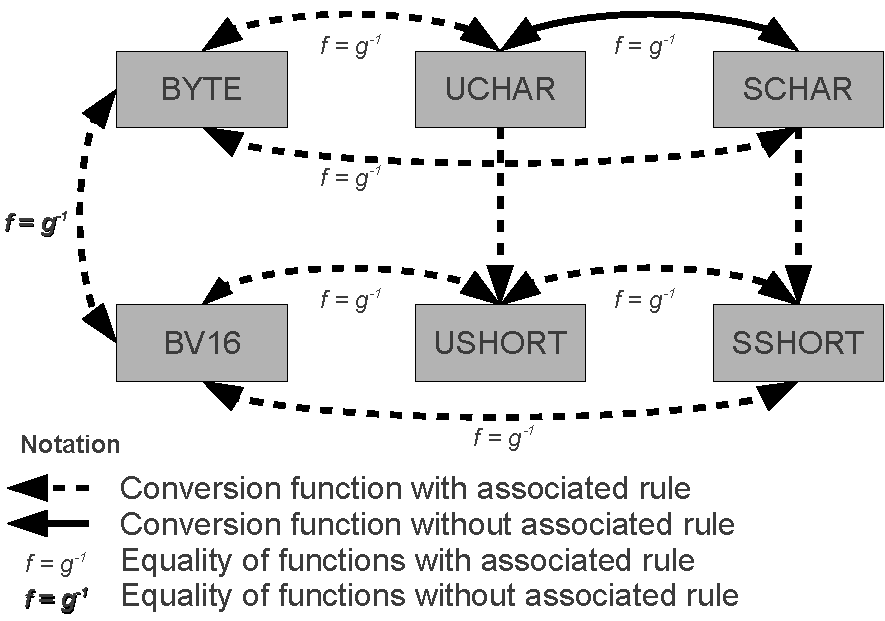
\includegraphics[width=3.in]{images/Diagram_Types_and_Rules.pdf}
\caption{Conversion functions}
\label{DiagramTypesRules}
\end{figure}


The conversion functions need to satisfy two properties: bijectivity
and equality to the reverse of the dual conversion function. Three
such proof obligations were verified automatically with AtelierB: (\it
uchar\_schar\rm \ $\in$ \textit{UCHAR} $\bij$ \textit{SCHAR}), (\it
schar\_uchar\rm \ $\in$ \textit{SCHAR} $\bij$ \textit{UCHAR}) and (\it
byte\_bv16\rm \ $=$ \it bv16\_byte\rm $^{-1}$).
%\begin{enumerate}
%
%\item (\it uchar\_schar\rm \ $\in$ \textit{UCHAR} $\bij$ \textit{SCHAR})
%\item (\it schar\_uchar\rm \ $\in$ \textit{SCHAR} $\bij$ \textit{UCHAR})
%\item (\it byte\_bv16\rm \ $=$ \it bv16\_byte\rm $^{-1}$) 
%
%\end{enumerate}
For the remaining proof obligations, we again had to create new proof
rules. There are three kinds of proof rules, that we illustrate by giving
one example each:

%Four conditions are needed to be a bijective function:
%
%\begin{description}
%\item $func$ is a function:\\
%$\forall$ \rm (\it xx\rm ,\it yy\rm ,\it zz\rm )\rm .\rm ( \it xx  $\in$  \bf dom\rm (\it func\rm )  $\land$  \it yy $\in$  \bf ran\rm (\it func\rm )  $\land$ \\ \it zz $\in$  \bf ran\rm (\it func\rm )  $\land$ \rm ( \it xx $\mapsto$  \it yy\rm )  $\in$  \it func  $\land$  \rm ( \it xx $\mapsto$  \it zz\rm )  $\in$  \it func  $\implies$  \it yy\rm =\it zz \rm )
%
%\item $func$ is an injective function:\\
%$\forall$ \rm (\it vv\rm ,\it xx\rm )\rm .\rm ( \it vv $\in$  \bf dom\rm (\it func\rm )  $\land$  \it xx  $\in$  \bf dom\rm (\it func\rm )  $\implies$  \it func\rm (\it vv\rm )\rm =\it func\rm (\it xx\rm ) \rm )
%
%\item $func$ is a total function:\\
%$\forall$ \it xx\rm .\rm ( \it xx  $\in$  \bf dom\rm (\it func\rm )  $\implies$   $\exists$ \it yy\rm .\rm ( \it yy  $\in$  \bf ran\rm (\it func\rm )  $\land$  \it func\rm (\it xx\rm )\rm =\it yy \rm )\rm ) 
%
%\item $func$ is surjective function:\\
% $\forall$ \it yy\rm .\rm ( \it yy $\in$  \bf ran\rm (\it func\rm ) $\implies$   $\exists$ \it xx\rm .\rm ( \it xx  $\in$  \bf dom\rm (\it func\rm ) $\land$  \it func\rm (\it xx\rm )\rm =\it yy \rm )\rm ) 
%
%
%\end{description} 
%
%Here, two conversion functions between bit vectors and the natural are presented. These functions are finite and convert from \textit{BYTE} to \textit{UCHAR} and vice versa.\textit{UCHAR} is a range between 0 and 255 and \textit{BYTE} is a bit vector with eight elements enumerated starting from 1. We need to prove that $byte\_uchar$  and $uchar\_byte$  are bijective functions and  $byte\_uchar = uchar\_byte^{-1}$. These functions are defined as follows:
%\begin{description}
%
%
%\item\it byte\_uchar \rm = $\lambda$  \rm ( \it v0 \rm ) \rm . \rm ( \it v0  $\in$  \it BYTE  $\mid$ \hspace*{0.10in}\it 2$^{7}$ $\times$ \it v0\rm (\rm 8\rm )\rm +\it 2$^{6}$  $\times$ \it v0\rm (\rm 7\rm )\rm + \it 2$^{5}$ $\times$ \it v0\rm (\rm 6\rm )\rm +\it 2$^{4}$ $\times$ \it v0\rm (\rm 5\rm ) \rm + \it 2$^{3}$  $\times$  \it v0\rm (\rm 4 \rm ) \rm + \it 2$^{2}$  $\times$ \it v0\rm (\rm 3\rm ) \rm + \it 2$^{1}$  $\times$  \it v0\rm (\rm 2\rm ) \rm + \it 2$^{0}$  $\times$  \it v0\rm (\rm 1\rm )\rm) 
%
%\item\it uchar\_byte \rm = $\lambda$  \rm ( \it v0 \rm ) \rm . \rm ( \it v0  $\in$  \it UCHAR $\mid$ \rm [\rm (\it v0   $\mod$ \it 2$^{1}$\rm ) $\div$ \it 2$^{0}$\rm , \rm (\it v0  $\mod$  \it 2$^{2}$\rm ) $\div$ \it 2$^{1}$\rm , \rm (\it v0  $\mod$  \it 2$^{3}$\rm ) $\div$ \it 2$^{2}$\rm , \rm (\it v0  $\mod$  \it 2$^{4}$\rm ) $\div$ \it 2$^{3}$\rm , \rm (\it v0  $\mod$  \it 2$^{5}$\rm ) $\div$ \it 2$^{4}$\rm , \rm(\it v0  $\mod$  \it 2$^{6}$\rm ) $\div$ \it 2$^{5}$\rm ,\rm (\it v0  $\mod$  \it 2$^{7}$\rm ) $\div$ \it 2$^{6}$\rm , \rm (\it v0  $\mod$  \it 2$^{8}$\rm ) $\div$ \it 2$^{7}$\rm \rm ] \rm)
%
%\end{description}
%
%The equivalent definitions using B sequence notation and set notation are:\\
%\it uchar\_byte \rm = \rm \{ \rm 0 $\mapsto$ \rm \rm [\rm 0\rm ,\rm 0\rm ,\rm 0\rm ,\rm 0\rm ,\rm 0\rm ,\rm 0\rm ,\rm 0\rm ,\rm 0\rm \rm ]\rm, \ldots  , \rm 2\rm 5\rm 5 $\mapsto$ \rm \rm [\rm 1\rm ,\rm 1\rm ,\rm 1\rm ,\rm 1\rm ,\rm 1\rm ,\rm 1\rm ,\rm 1\rm ,\rm 1\rm \rm ]\rm \}  \\
%\it byte\_uchar \rm =  \rm \{\rm \rm [\rm 0\rm ,\rm 0\rm ,\rm 0\rm ,\rm 0\rm ,\rm 0\rm ,\rm 0\rm ,\rm 0\rm ,\rm 0\rm \rm ] $\mapsto$ \rm 0\rm, \ldots , \rm \rm [\rm 1\rm ,\rm 1\rm ,\rm 1\rm ,\rm 1\rm ,\rm 1\rm ,\rm 1\rm ,\rm 1\rm ,\rm 1\rm \rm ] $\mapsto$ \rm 2\rm 5\rm 5 \rm \} \rm 
%
%\paragraph{B Rules:}
%These rules represent that  $byte\_uchar$  and $uchar\_byte$  are bijective functions and  $byte\_uchar = uchar\_byte^{-1}$. These rules are used on interactive prover of Atelierb.



\begin{enumerate}

\item For the proof obligation (\it byte\_uchar\rm \ $\in$ \textit{BYTE} $\bij$
\textit{UCHAR}), the proof rule is:\\
$\lambda$ \it v0\rm .\rm (\it v0 $\in$  \rm 1 $\upto$ \rm 8  $\fun$  \rm \{\rm 0\rm ,\rm 1\rm \}  $\mid$  \rm 1\rm 2\rm 8 $\times$ \it v0\rm (\rm 8\rm )\rm +\rm 6\rm 4 $\times$ \it v0\rm (\rm 7\rm )\rm +\rm 3\rm 2 $\times$ \it v0\rm (\rm 6\rm )\rm +\rm 1\rm 6 $\times$ \it v0\rm (\rm 5\rm )\rm +\rm 8 $\times$ \it v0\rm (\rm 4\rm )\rm +\rm 4 $\times$ \it v0\rm (\rm 3\rm )\rm +\rm 2 $\times$ \it v0\rm (\rm 2\rm )\rm +\rm 1 $\times$ \it v0\rm (\rm 1\rm )\rm ) \rm $\in$ \rm (\rm 1 $\upto$ \rm 8  $\fun$  \rm \{\rm 0\rm ,\rm 1\rm \}\rm )  $\bij$  \rm 0 $\upto$ \rm 2\rm 5\rm 5 \\

\item For the proof obligation (\it uchar\_byte\rm \ $\in$ \textit{UCHAR} $\bij$
\textit{BYTE}), the proof rule is:\\ $\lambda$ \it v0\rm .\rm (\it v0 $\in$  \rm 0$\upto$255  $\mid$  \rm \rm  [(\it v0  $\mod$  \rm 2)$\div$1,(\it v0  $\mod$  \rm 4)$\div$\rm 2\rm,(\it v0  $\mod$  \rm 8)$\div$\rm 4\rm,(\it v0  $\mod$  \rm 16)$\div$\rm 8\rm,(\it v0  $\mod$  \rm 32)$\div$\rm 1\rm 6\rm,(\it v0  $\mod$  \rm 6\rm 4)$\div$\rm 3\rm 2\rm,(\it v0  $\mod$  \rm 1\rm 2\rm 8)$\div$\rm 6\rm 4\rm,(\it v0  $\mod$  \rm 2\rm 5\rm 6)$\div$\rm 1\rm 2\rm 8\rm \rm ]\rm ) \rm   $\in$  \rm 0 $\upto$ \rm 2\rm 5\rm 5   $\bij$ \rm (\rm 1 $\upto$ \rm 8  $\fun$  \rm \{\rm 0\rm ,\rm 1\rm \}\rm )\\


\item For the proof obligation (\it byte\_uchar\rm  =  \it
uchar\_byte\rm$^{-1}$), the proof rule is:\\ $\lambda$ \it v0\rm .\rm (\it v0 $\in$  \rm 1 $\upto$ \rm 8  $\fun$  \rm \{\rm 0\rm ,\rm 1\rm \}  $\mid$  \rm 1\rm 2\rm 8 $\times$ \it v0\rm (\rm 8\rm )\rm +\rm 6\rm 4 $\times$ \it v0\rm (\rm 7\rm )\rm +\rm 3\rm 2 $\times$ \it v0\rm (\rm 6\rm )\rm +\rm 1\rm 6 $\times$ \it v0\rm (\rm 5\rm )\rm +\rm 8 $\times$ \it v0\rm (\rm 4\rm )\rm +\rm 4 $\times$ \it v0\rm (\rm 3\rm )\rm +\rm 2 $\times$ \it v0\rm (\rm 2\rm )\rm +\rm 1 $\times$ \it v0\rm (\rm 1\rm )\rm )=($\lambda$ \it v0\rm .\rm (\it v0 $\in$  \rm 0$\upto$255  $\mid$  \rm \rm  [(\it v0  $\mod$  \rm 2)$\div$1,(\it v0  $\mod$  \rm 4)$\div$\rm 2\rm,(\it v0  $\mod$ \rm 8) $\div$\rm 4\rm,(\it v0  $\mod$  \rm 16)$\div$\rm 8\rm,(\it v0  $\mod$  \rm 32)$\div$\rm 1\rm 6\rm,(\it v0  $\mod$ \rm 6\rm 4)$\div$\rm 3\rm 2\rm,(\it v0  $\mod$  \rm 1\rm 2\rm 8)$\div$\rm 6\rm 4\rm,(\it v0  $\mod$  \rm 2\rm 5\rm 6)$\div$\rm 1\rm 2\rm 8\rm \rm ]\rm )\rm)$^{-1}$
\end{enumerate}

Eight proof obligations require that conversion functions are finite. %: \it
% byte\_uchar $\in$ $\finset$\rm (\it byte\_uchar\rm ); \it uchar\_byte  $\in$
% $\finset$\rm (\it uchar\_byte\rm ); \it ushort\_bv16 $ \in \finset$\rm (\it
% ushort\_bv16\rm ); \it bv16\_ushort $ \in \finset$\rm (\it bv16\_ushort\rm ); \it
% byte\_schar $ \in \finset$\rm (\it byte\_schar\rm ); \it schar\_byte $ \in
% \finset$\rm (\it schar\_byte\rm ); \it sshort\_bv16 $ \in \finset$\rm (\it
% sshort\_bv16\rm ); and \it bv16\_sshort $ \in \finset$\rm (\it bv16\_sshort\rm).
 These proof obligations were verified using the expression evaluator of ProB.
Finally, we have included rules related to binary arithmetic as developed
in~\cite{Leibnizens}. These rules are used in the interactive theorem prover with
binary arithmetic to prove important properties~\cite{James2010,Dasgupta2006}.



\section{A B model of the Z80 instruction set}
\label{sec:z80}

The \textit{Z80} is a CISC microcontroller developed by
\textit{Zilog}~\cite{Z80_manual}. The Z80 is composed by different
elements and a simplified internal organization is shown in the Figure
\ref{fig:DiagramBlock}.  This figure has some important elements of
Z80 CPU: ALU, registers of 8 and 16 bits and input/output ports.

\begin{figure}[h] \centering
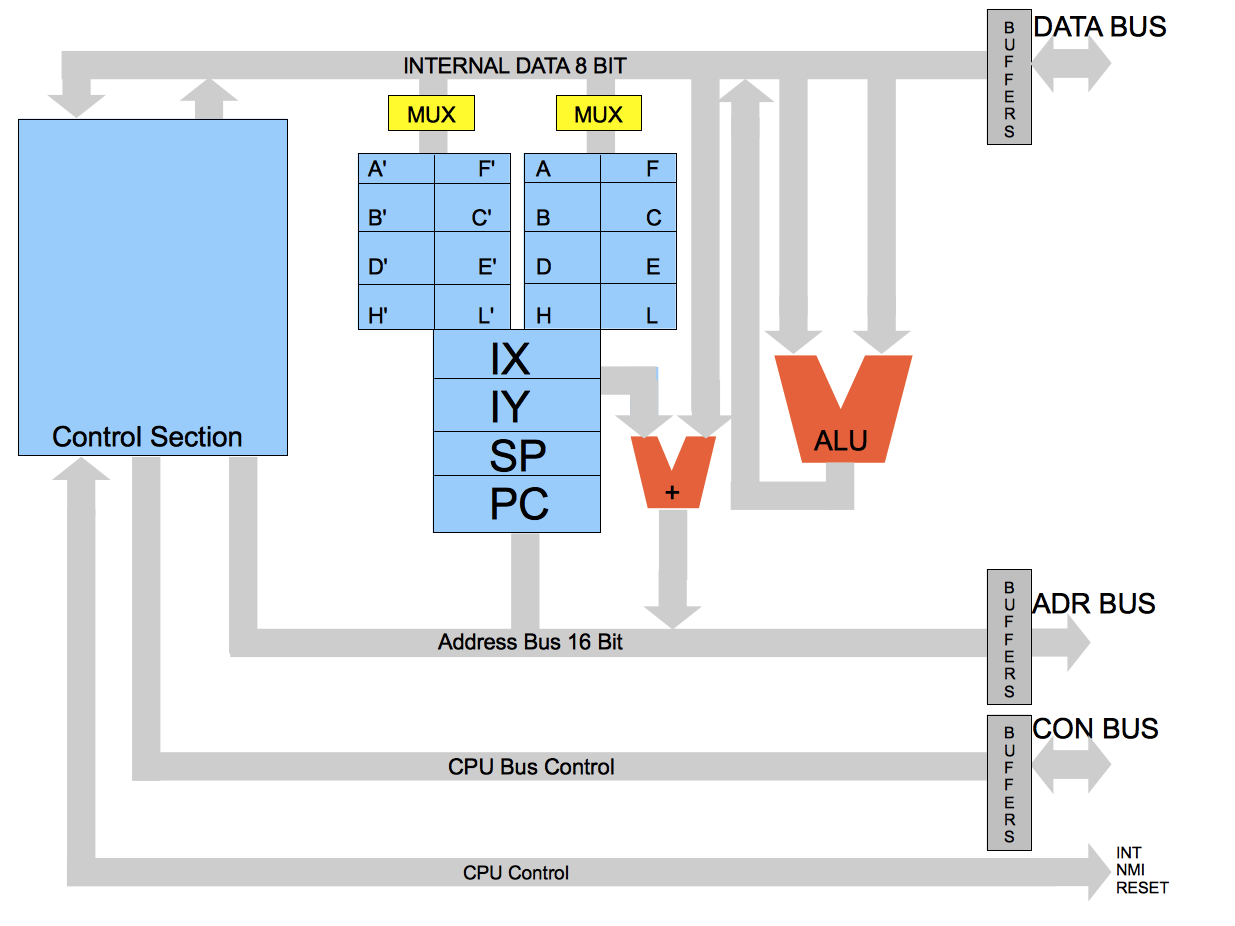
\includegraphics[width=0.70\textwidth]{images/Architecture.png}
\caption{Simplified internal organization of Z80 CPU.}
\label{fig:DiagramBlock}
\end{figure}


The Z80 has 158 different instructions, including all the 78 from the Intel 8080
microprocessor, and all of them were formally specified in B. These instructions are classified
into these categories: load and exchange; block transfer and search; arithmetic
and logical; rotate and shift; bit manipulation; jump, call and return;
input/output; and basic cpu control. Each category of instruction has different
elements of specification.


This section shows the elements that make up the different types of
instructions. The main elements are specified in the microcontroller module Z80
and parts of it are presented below.  Basically, the state of microcontroller is
formed by data from program counter, ports, registers, etc. The transitions
between the states are actioned by execution of instruction or an external
action. Groups of registers are represented by the variables of the
specification states that appear in clause \textit{VARIABLES}. The declaration
of valid states of variables is in the \textit{INVARIANT} clause and the initial
state is defined in the \textit{INITIALISATION} clause. The assembly
instructions are defined by the clause \textit{OPERATIONS} and, in general, each
instruction has three actions: update the program counter, update the flag
register and its main effect.
% Several functions were created to Z80.
General functions that can be used in other microcontroller models are defined
in the modules of data types. Specific functions of the microcontroller are
defined in the ALU (arithmetic logic unit) module.



The main module includes an instance of the memory module and accesses the
definitions from basic data types modules and the \textit{ALU} module.

	\begin{center}
	\begin{sloppypar}
	
	  \begin{tabbing}
	    \begin{array}[t]{l}
		\bf MACHINE\\
		\hspace*{0.15in}\it Z80\\
		\bf INCLUDES\\
		\hspace*{0.10in}\it MEMORY
	    \end{array}
	     \hspace*{1cm} 
	    \begin{array}[t]{l}
	    \bf SEES\\
		\hspace*{0.10in}\it ALU, \it BIT\_DEFINITION, \it BIT\_VECTOR\_DEFINITION,\\
		\hspace*{0.10in}\it BYTE\_DEFINITION, \it BV16\_DEFINITION,\\
		\hspace*{0.10in}\it UCHAR\_DEFINITION, \it SCHAR\_DEFINITION,\\
		\hspace*{0.10in}\it SSHORT\_DEFINITION ,\it USHORT\_DEFINITION\\
	    \end{array}
	  \end{tabbing}
	  
	 \end{sloppypar} 
	\end{center}


\subsection{Modeling registers}

The Z80 CPU includes alternative set of accumulator, flag and general registers.
The CPU contains a stack pointer ($\textit{sp}$), program counter
($\textit{pc}$), two index registers ($\textit{ix}$ and $\textit{iy}$), an
interrupt register ($\textit{i\_}$), a refresh register ($\textit{r\_}$), two
bits ($\textit{iff1}$, $\textit{iff2}$) used to control the interruptions, a
pair of bits to define the interruption mode ($\textit{im}$) and the input and
output ports ($\textit{i\_o\_ports}$). These definitions are represented by
\textit{INVARIANT}.
  

\begin{sloppypar}
\bf INVARIANT

\hspace*{0.10in}\it rgs8  $\in$  \it id\_reg\_8  $\fun$  \it BYTE  $\land$ \it pc  $\in$  \it INSTRUCTION  $\land$  \it sp  $\in$  \it BV16 $\land$  \it ix  $\in$  \it BV16  $\land$

\hspace*{0.10in}\it iy  $\in$  \it BV16  $\land$ \it i\_  $\in$  \it BYTE  $\land$  \it r\_ $\in$  \it BYTE  $\land$ \it iff1  $\in$  \it BIT  $\land$ \it iff2  $\in$  \it BIT  $\land$ 

\hspace*{0.10in}\it im $\in$ (\it BIT $\times$ \it BIT\rm )  $\land$  \it i\_o\_ports  $\in$  \it BYTE  $\fun$  \it BYTE
\end{sloppypar}


 

% Features of microcontroller
The internal registers contains 176 bits of read/write memory that are
represented by identifiers used as parameters in the instructions . It includes
two sets of six general purpose registers which may be used individually as
8-bit registers or as 16-bit register pairs.  The working registers are
represented by variable $\textit{rgs8}$. The domain of $\textit{rgs8}$
($\textit{id\_reg8}$) is a set formed by identifiers of registers of 8 bits.
These registers are called main register set (\textit{a0,b0,c0,d0,e0,f0,h0,l0})
and alternate register set (\textit{a\_0,b\_0,c\_0,d\_0,e\_0,f\_0,h\_0,l\_0}).
These registers can be accessed in pairs, forming 16-bits, resulting in another
set of identifiers of 16-bits registers, named $\textit{id\_reg16}$. These sets
are represented below.

\begin{sloppypar}

	\bf SETS\\
\hspace*{0.10in}\it id\_reg\_8 \rm = \rm \{ \it a0\rm, \it f0\rm, \it b0\rm, \it
c0\rm, \it d0\rm, \it e0\rm, \it h0\rm, \it l0\rm, \it a\_0\rm,  \it f\_0\rm,
\it b\_0\rm, \it c\_0\rm, \it d\_0\rm, \it e\_0\rm, \it h\_0\rm, \it l\_0 \rm
\};\\ \hspace*{0.10in}\it id\_reg\_16 \rm = \rm \{  \it AF \rm, \it BC\rm, \it
DE\rm, \it HL\rm, \it SP\rm\}
	

\end{sloppypar}

%\begin{sloppypar}
%
%	\bf SETS\\
%	\hspace*{0.10in}\it id\_reg\_8 \rm = \rm \{ \it a0 \rm , \it f0 \rm , \it f\_0 \rm , \it a\_0 \rm ,\\
%	\hspace*{0.93in}\it b0 \rm , \it c0 \rm , \it b\_0 \rm , \it c\_0\rm,\\
%	\hspace*{0.93in}\it d0 \rm , \it e0 \rm , \it d\_0 \rm , \it e\_0\rm,\\
%	\hspace*{0.93in}\it h0 \rm , \it l0 \rm , \it h\_0 \rm , \it l\_0\};\\
%	\hspace*{0.10in}\it id\_reg\_16 \rm = \rm \{ \it BC \rm , \it DE \rm , \it HL \rm , \it SP \rm , \it AF \rm \}
%\end{sloppypar}


The main working register of Z80 is the accumulator ($\textit{rgs8(a0)}$) used for arithmetic/logic, input/output and loading/storing operations.
Another important element is the ``f'' register ($\textit{rgs8(f0)}$),  that is
used as a \textbf{flag register}. This register uses only six bits to represent the execution result status of each instruction.
According to the official manual the bits 3 and 5 are not used and the others bits have the follow meaning: %$\textit{bv\_get(rgs8(f0),0)}$ - the carry bit; $\textit{bv\_get(rgs8(f0),1)}$ - the add/subtract bit; $\textit{bv\_get(rgs8(f0),2)}$ - the parity or overflow bit; $\textit{bv\_get(rgs8(f0),4)}$ - the half carry bit; $\textit{bv\_get(rgs8(f0),6)}$ - the zero bit; and $\textit{bv\_get(rgs8(f0),7)}$ - the sign bit.
\begin{description}
  \item[$\textit{bv\_get(rgs8(f0),0)}$] - The Carry bit.
  \item[$\textit{bv\_get(rgs8(f0),1)}$] - The Add/Subtract bit.
  \item[$\textit{bv\_get(rgs8(f0),2)}$] - The Parity or Overflow bit.
  \item[$\textit{bv\_get(rgs8(f0),4)}$] - The Half Carry bit.
  \item[$\textit{bv\_get(rgs8(f0),6)}$] - The Zero bit.
  \item[$\textit{bv\_get(rgs8(f0),7)}$] - The Sign bit.
\end{description}
These bits can also be used to specify security properties for microcontroller programs.   

\textbf{Assuring the absence of overflow:}
 \emph{To assure that an overflow does not happen, the developer can add this
 expression (\textit{bv\_get(rgs8(f0),0)} $\neq$ 1 $\land$
 \textit{bv\_get(rgs8(f0),2) $\neq$ 1}) in the invariant.
% When a overflow happen,it can be dangerous. So the developer may restrict its use. However, this restriction can also
% become more difficult to verify the model.
}

\subsection{Manipulation data functions from Z80}

 There are some specific functions from Z80 to manipulate the data. In addressing mode, the function
$\textit{bv\_ireg\_plus\_d}$ receives the value of a register ($\textit{ix}$ or $\textit{iy}$) 
used as a base to point to a region in memory from which data is to be stored or retrieved.
%and the displacement to return the sum, the result is the dislocated address memory, 
 An additional byte is included in indexed instructions to specify an offset from this base. This displacement is specified as a two's complement signed integer. This function is defined as:\\

\hspace*{0.0in}\it bv\_ireg\_plus\_d \rm : \rm(\it BV16  $\times$  \it SCHAR  $\fun$  \it BV16\rm )  $\land$ 

\hspace*{0.0in}\it bv\_ireg\_plus\_d \rm =  $\lambda$  \rm ( \it ix\_iy \rm , \it offset \rm ) \rm . \rm ( \it ix\_iy  $\in$  \it BV16  $\land$  \it offset  $\in$  \it SCHAR   

\hspace*{0.20in}$\mid$ \it ushort\_bv16 \rm ( \rm (\it bv16\_ushort \rm ( \it ix\_iy \rm ) \rm + \it offset \rm ) 
\textbf{\textit{mod}} $2^{16}$ ) \rm )\\

Another derived function is  $\textit{bv\_(ireg\_plus\_d)}$, which returns the value in the memory  address
returned by the $\textit{bv\_ireg\_plus\_d}$ function and its definition is similar.

There is a specific function to refresh the flag register, it is named $\textit{update\_reg\_flag}$. It is typed and defined as follow:\it update\_flag\_reg \rm $\in$ \rm (\it BIT  $\times$  \it BIT  $\times$  \it BIT  $\times$  \it
BIT $\times$  \it BIT  $\times$  \it BIT\rm) $\fun$  \rm (\rm \{\it f0\rm \}  $\times$  \it BYTE\rm ).  This function is defined as:\\

 \it update\_flag\_reg \rm =  $\lambda$  \rm (\it s7 \rm, \it z6 \rm,\it h4 \rm,\it pv2 \rm ,\it n1
\rm ,\it c0 \rm) . 
\rm ( \it s7 $\in$ \it BIT $\land$ \it z6 $\in$ \it BIT $\land$ \it h4 $\in$ \it BIT $\land$ \it pv2 $\in$ \it BIT $\land$ \it n1 $\in$ \it BIT $\land$ \it c0 $\in$ \it BIT \rm $\mid$( \it f0  $\mapsto$ \rm [\it c0\rm , \it n1\rm , \it pv2\rm , \rm 1\rm , \it h4\rm , \rm 1\rm , \it z6\rm , \it s7\rm \rm ]\rm ) \rm )


\subsection{Program, stack and data memory}

The Z80 uses a unique memory for storing program instructions, data stack and
general-purpose data. The memory has 16-bit addresses and each address holds a byte.
Thus, the memory is very simple: \it mem  $\in$  \it BV16  $\fun$  \it BYTE\rm.
 
In general, the instructions can access all memory addresses, but it is dangerous. The user may mistakenly
access and change data in memory. For added  security, it is important that the program instructions has
limited access by region. Thus the designer can specify address regions in a refinement model to restrict the access from
instructions. The address regions can be specified using constants
($\textit{PROGRAM\_R\_ADR,DATA\_R\_ADR,STACK\_R\_ADR}$), these define respectively a range of restricted
address for: programs instructions, general purpose data and data stack.
%
%$
%\begin{array}{l}
%\textit{PROGRAM\_R\_ADR} = 0..16384 \land\\
%\textit{DATA\_R\_ADR} = 16385..49151 \land\\
%\textit{STACK\_R\_ADR} = 49152..65535
%\end{array}
%$

\textbf{Assuring the absence of overlapping of address regions:}
 \emph{To assure that address regions are well defined, then the designer must verify the expression:}
%\begin{sloppypar}
%\hspace*{0.10in}
\it PROGRAM\_R\_ADR $\cap$ DATA\_R\_ADR $\cap$ $=$ \{\} $\land$ STACK\_R\_ADR $\cap$ DATA\_R\_ADR $\cap$ $=$ \{\} $\land$ PROGRAM\_R\_ADR $\cap$  STACK\_R\_ADR  $=$ \{\} \rm
%\end{sloppypar}
 
\textbf{Preserving the memory consistency:} \emph{In general, the access to
some address regions is dangerous. Then, each instruction has a specific pre-condition that verifies
if the new address memory, that will be updated, is a member of its region. For example, the $\textit{PUSH}$
program instruction permits write only in the region of stack ($\textit{STACK\_R\_ADR}$\rm).}



\subsection{Arithmetic logic unit}
 
There are many functions in the module \textit{ALU}. In general, the definition of these 
functions use basic definitions or previously defined functions. For example, the function
$\textit{half8UCHAR}$ is used to get the half part of $\textit{UCHAR}$ value.
It is important to know the half carry and it is used in the function $\textit{add8UCHAR}$. \\

\hspace*{0.0in}\it half8UCHAR  $\in$  \it UCHAR  $\fun$  \it UCHAR  $\land$ 

\hspace*{0.0in}\it half8UCHAR \rm =  $\lambda$  \rm (\it ww\rm )\rm .\rm (\it ww  $\in$  \it UCHAR  $\mid$  \it ww  $\mod$  \it $2^{4}$\rm )\\


 
The function $\textit{add8UCHAR}$ receives a bit carry and two $\textit{UCHAR}$ values and returns respectively the 
sum, the sign bit, the carry bit, the half carry bit and the zero bit. It is typed as follows: \it add8UCHAR \rm :
\rm (\it BIT $\times$ \it UCHAR $\times$ \it UCHAR\rm ) $\fun$ \rm (\it UCHAR $\times$  \it BIT  $\times$  \it BIT  $\times$  \it BIT  $\times$  \it BIT\rm ) and its definition is:\\

\hspace*{0.0in}\it add8UCHAR\rm = $\lambda$ \rm(\it carry\rm,\it w1\rm, \it w2\rm)\rm.\rm

\hspace*{0.0in}(\it carry $\in$  \it BIT  $\land$  \it w1  $\in$  \it UCHAR  $\land$  \it w2  $\in$  \it UCHAR
$\mid$

\hspace*{0.40in}\rm(\rm(\rm(\it carry \rm + \it w1 \rm + \it w2 \rm )  $\mod$  \it $2^{8}$ \rm ),

\hspace*{0.40in}\it bool\_bit\rm ( \it carry \rm + \it uchar\_schar\rm (\it w1\rm ) \rm + \it uchar\_schar \rm (\it
w2\rm ) $<$ \rm 0\rm ),

\hspace*{0.40in}\it bool\_bit\rm ( \it carry \rm + \it w1 \rm + \it w2 $>$ \it UCHAR\_MAX\rm )\rm ,

\hspace*{0.40in}\it bool\_bit\rm ( \it carry \rm + \it half8UCHAR\rm (\it w1\rm) \rm + \it half8UCHAR\rm (\it w2\rm)  $\geq$  \it $2^{4}$\rm )\rm,

\hspace*{0.40in}\it bool\_bit\rm ( \rm ( \rm (\it carry \rm + \it w1 \rm + \it w2 \rm )  $\mod$  \it $2^{8}$ \rm
)\rm = \rm 0\rm )\rm )\hspace*{0.10in}\rm )\\



A related function to subtract operation is $\textit{subtract8UCHAR}$. There are the same functions for the
$\textit{SCHAR}$ type, they are respectively $\textit{add8SCHAR}$ and $\textit{subtract8SCHAR}$, all these
functions are of 8 bits ($\textit{BYTE}$) and defined similarly. In the same way, the arithmetic functions for 16
bits ($\textit{BV16}$) are defined.
The module ALU has several others functions, for example:%but only some simplest functions also are explained below:
%\begin{itemize}
  %\item \it inc  $\in$ \it BYTE $\fun$  \it BYTE \rm - It receives a byte and
  %returns its increment. There is a similar function named $\textit{dec}$.
%  \item 
\it instruction\_next  $\in$  USHORT  $\fun$  USHORT \rm - It receives the  
  actual value from program counter register (\textit{pc}) and returns its increment;
% \item 
and \it is\_negative  $\in$  \it BYTE  $\fun$  \it BIT \rm - It returns the most significant bit,
 in other words, the signal bit.
  % \item \it is\_zero  $\in$  \it BYTE  $\fun$  \it BIT \rm - It returns 1 if the received
 % byte is zero, otherwise returns 0.
  %\item \it update\_refresh\_reg \rm - It receives a byte and returns its increment until the seventh bit.
%\end{itemize}
As the logic functions that are defined in the \textit{BYTE} and \textit{BV16}
module are included in the \textit{ALU} module, they can be seen and used
directly in the \textit{ALU} and \textit{Z80} modules.

\subsection{Modeling the actions and instructions}

Each instruction is represented by a B operation in Z80 module. The main
module (\textit{Z80}) has three categories of operations: a category represents the 
instructions of microcontrollers, a second category represents the input and output of data 
(shown in ~\ref{sec:modelingIO}) and the last category represents the external
actions (shown in~\ref{sec:externalactions}). A simple example of instruction is
$\textit{LD\_(nn)\_A}$\footnoteremember{myfootnote}{The B tools does not allow
to use parentheses in identifiers, and the characters \{``('',``)''\} are
replaced respectively by \{``9'',``0''\} in the actual specification.} shown below. The
pre-defined functions are necessary many times to model the instructions, these
functions facilitate the construction of instruction set model. By default, all
parameters in operations are either predefined elements in the model or
integers values in decimal representation. This instruction use the
$\textit{updateAddressMem}$ operation from \textit{Memory} module and it receives
a address memory and its new memory value. It also increments the program
counter ($\textit{pc}$) and update the refresh register ($\textit{r\_}$).
The other instructions have a similar structure.

\hspace*{0.00in}\bf LD\_9nn0\_A \rm ( \it nn \rm ) \rm =

\hspace*{0.20in}\bf PRE \it nn $\in$ \it USHORT\hspace*{0.15in} $\land$ \hspace*{0.10in}\it nn\hspace*{0.10in} $\in$  \it DATA\_R\_ADR \hspace*{0.10in}\bf THEN

\hspace*{0.20in}\bf updateAddressMem \rm ( \it ushort\_bv16 \rm ( \it nn \rm ) \rm , \it rgs8 \rm ( \it a0 \rm )
\rm )  $\para$

\hspace*{0.20in}\it pc \rm := \it instruction\_next \rm ( \it pc \rm )  $\para$  \it r\_ \rm := \it update\_refresh\_reg\rm (\it r\_\rm )

\hspace*{0.00in}\bf END\rm 



\subsection{Modeling the input/output instructions}
\label{sec:modelingIO}
The Z80 has an extensive set of input and output (I/O) instructions and 256 ports for
devices. This model can transfer data blocks between the I/O devices and any
of the internal registers or memory address.

The $\textit{IN\_r(C)}$\footnoterecall{myfootnote} instruction is represented
by the following B operation. It receives a register identifier ``$\textit{rr}$'' and, it stores the value from ``rr'' in the $\textit{C}$ port address. Besides, it increments the program counter and updates the flag registers.

\hspace*{0.0in}\bf IN\_r\_9C0 \rm ( \it rr \rm ) \rm =

\hspace*{0.0in}\bf PRE \it rr  $\in$  \it id\_reg\_8  $\land$  \it rr  $\not =$  \it f0\hspace*{0.15in}\bf THEN

\hspace*{0.20in}\bf ANY \hspace*{0.10in}\it negative \rm , \it zero \rm , \it half\_carry \rm , \it pv \rm , \it add\_sub \rm , \it carry

\hspace*{0.20in}\bf WHERE 

\hspace*{0.40in}\it negative $\in$ \it BIT $\land$ \it zero $\in$ \it BIT $\land$ \it half\_carry $\in$ \it BIT 
$\land$ \it pv $\in$ \it BIT $\land$

 \hspace*{0.40in}\it add\_sub $\in$ \it BIT $\land$ \it carry $\in$ \it BIT  $\land$

\hspace*{0.40in}\it negative \rm = \it is\_negative \rm ( \it io\_ports \rm ( \it rgs8 \rm ( \it c0 \rm ) \rm ) \rm )  $\land$ 

\hspace*{0.40in}\it zero \rm = \it is\_zero \rm ( \it io\_ports \rm ( \it rgs8 \rm ( \it c0 \rm ) \rm ) \rm )  $\land$ \it half\_carry \rm = \rm 0  $\land$ 

\hspace*{0.40in}\it pv \rm = \it parity\_even \rm ( \it io\_ports \rm ( \it rgs8 \rm ( \it c0 \rm ) \rm ) \rm ) $\land$
\it add\_sub \rm =\hspace*{0.10in}\rm 0  $\land$ 
\it carry \rm = \it z\_c

\hspace*{0.20in}\bf THEN

\hspace*{0.40in}\it rgs8 \rm := \it rgs8  $\lover$  \rm \{ \rm ( \it rr  $\mapsto$  \it io\_ports \rm ( \it rgs8 \rm ( \it c0 \rm ) \rm ) \rm ) \rm ,

\hspace*{0.40in}\it update\_flag\_reg\rm (\it negative\rm,\it zero\rm,\it half\_carry\rm,\it pv\rm,\it add\_sub\rm,\it carry)\rm\}$\para$

\hspace*{0.40in}\it pc \rm := \it instruction\_next \rm ( \it pc \rm )  $\para$  \it r\_ \rm := \it update\_refresh\_reg\rm (\it r\_\rm )

\hspace*{0.20in}\bf END

\hspace*{0.0in}\bf END \rm

%The main I/O instructions work similarly, for example: $\textit{OUT(n),A}$  or $\textit{OUT (C ), r}$. 

% $
% \begin{array}{l} 
% \textit{IN\_r\_9C0} ( rr ) = \\
% \quad   \PRE rr \in id\_reg\_8    \THEN\\
% \quad\quad \ANY data\_in, negative , zero , half\_carry , pv , add\_sub , carry\\ 
% \quad\quad \WHERE data\_in \in \textit{BYTE} \land negative \in \textit{BIT}\land\\
% \quad\quad\quad carry \in \textit{BIT} \land half\_carry \in \textit{BIT} \land zero \in \textit{BIT} \land \\
% \quad\quad\quad negative = is\_negative (data\_in) \land zero = is\_zero(data\_in ) \land\\
% \quad\quad\quad half\_carry = 0 \land pv =parity\_even\_BYTE ( data\_in )    \land\\
% \quad\quad\quad add\_sub =  0 \land carry = z\_c \\
% \quad\quad  \THEN \\
% \quad\quad\quad i\_o\_ports ( rgs8 ( c0 ) ) := data\_in ||\\
% \quad\quad\quad rgs8 := rgs8 <+ \{ ( rr |-> data\_in ) ,\\
% \quad\quad\quad get\_new\_flag\_register\_SZ\_H\_PvNC ( rgs8 , negative , zero, half\_carry , pv , add\_sub , carry ) \} ||\\
% \quad\quad\quad pc := instruction\_next( pc )\\
% \quad\quad \END\\
% \quad \END\\
% \end{array}
% $




\subsection{Modeling the external actions}
\label{sec:externalactions}

The external actions change the state of the microcontroller, for example,
refreshing the I/O ports and interruption request. The external actions are also
modeled by operations and they are named with the prefix ``$ext\_$'' and
followed by the name of action. There are four external actions:
$ext\_update\_io\_ports$, $ext\_NMI$ and $ext\_INT$, $ext\_Reset$. The
instruction $ext\_update\_io\_ports$ just changes the state of I/O port, see.

\hspace*{0.20in}\bf ext\_update\_io\_ports\rm (\it address\rm ,\it value\rm )\rm =

\hspace*{0.20in}\bf PRE \it address  $\in$  \it UCHAR  $\land$ \hspace*{0.10in}\it value  $\in$  \it SCHAR \bf THEN

\hspace*{0.40in}\it io\_ports \rm ( \it uchar\_byte \rm ( \it address \rm ) \rm ) \rm := \it schar\_byte \rm ( \it
value \rm )

\hspace*{0.20in}\bf END\rm 

The other external actions are related to interruptions. Interruptions allow
devices to suspend a routine from CPU and start another service routine.
This service routine can exchange data or signals between CPU and external
devices. When a routine is finished, then the CPU comes back to the last routine
that was interrupted.

For the interrupts, the following elements are important:  the interrupt flip-flops
($\textit{iff1}$ and $\textit{iff2}$), the types of interrupts (maskable and
non-maskable), the interrupt mode (set with the $\textit{IM 0}$, $\textit{IM 1}$,
$\textit{IM 2}$ instructions) and the $\textit{i\_}$ register.

Flip-flops $\textit{iff1}$ and $\textit{iff2}$ control the maskable interrupts
($\textit{INT}$). When $\textit{iff1}$ is set, the interrupt is enabled,
otherwise it is disabled; $\textit{iff2}$ is used only as backup for $\textit{iff1}$. The
instructions $\textit{EI}$ and $\textit{DI}$ respectively enable and disable the
maskable interruptions, setting  $\textit{iff1}$ to 1 and 0.


The interruptions and the \textit{reset} action can change the state of program
counter. Theses actions are modeled by B operations and its main effects are
presented here\footnote{Some definitions of constants: $\textit{sp\_minus\_two}$
holds the value of stack pointer minus 2,
% =$\textit{dec\_BV16(dec\_BV16(sp))}$
 $\textit{sp\_minus\_one}$ is the value of stack pointer minus 1,
% =$\textit{dec\_BV16(sp)}$
$\textit{pc\_high}$ holds the most significant 8 bits and $\textit{pc\_low}$
holds the least significant 8 bits.}.


 \textbf{NMI} - Non-maskable interrupts cannot be disabled
 by the programmer. Then, when a device makes a request, $sp$ is pushed,
 $pc$ receives $66H$ (102 in decimal), $\textit{iff1}$ is reset, $\textit{iff2}$ stores
 $\textit{iff1}$ and the refresh register is updated.
  
\begin{sloppypar}
\bf updateStack\rm (\rm \{ \rm (\it sp\_minus\_two  $\mapsto$  \it pc\_low\rm )\rm ,\rm (\it sp\_minus\_one  $\mapsto$ \it pc\_high \rm ) \rm \}\rm )$\para$

\it sp \rm := \it sp\_minus\_two  $\para$ \it pc \rm := \rm 1\rm 0\rm 2 $\para$ \it iff1\rm :=\rm 0  $\para$  \it iff2\rm := \it iff1 $\para$

\it r\_ \rm := \it update\_refresh\_reg\rm (\it r\_\rm )\\
\end{sloppypar}

  \textbf{INT} - Maskable Interrupt is usually reserved for important functions
  that can be enabled and disabled by the programmer. When a maskable interrupt
  action happens, both $\textit{iff1}$ and $\textit{iff2}$ are cleared,
  disabling the interrupts, $sp$ is pushed, the refresh register is updated and
  the other effects depend on the interrupt mode register (\it im\rm).
 

 \begin{itemize}
   
  \item The mode 0 is compatible with 8080 and this mode is selected when \it im
  \rm = \rm ( \rm 0 $\mapsto$  \rm 0 \rm ). When a  non-maskable interrupt
  happens, the CPU fetches an instruction of one byte from an external device,
  usually an RST instruction, and the CPU executes it.
  The instruction code is received from an external device by data bus and it is
  represented by integer parameter called $\textit{byte\_bus}$.

 
  \item The mode 1 is the simplest and this mode is selected when \it im \rm =
  \rm ( \rm 0  $\mapsto$  \rm 1 \rm ). Simply, when a non-maskable interruption
  happens, the program counter receives $38H$ (56 in decimal).
  
  \item The mode 2 is the most flexible and this mode is selected when \it im
  \rm = \rm ( \rm 1  $\mapsto$ \rm 1 \rm ). When a non-maskable interruption
  happens, an indirect call can be made to any address memory. The program
  counter receives a bit vector of size 16 composed with two parts: the most
  significant part of the $\textit{i\_}$ register and the least significant part
  of the $\textit{byte\_bus}$ with the last bit cleared.
  
 \end{itemize}

The essential part of maskable interrupt is shown below, where
$\textit{byte\_bus}$ is a parameter of the $\textit{INT}$ operation:
 


\begin{sloppypar}

\hspace*{0.00in}\bf IF \it im \rm = \rm ( \rm 0  $\mapsto$  \rm 0 \rm ) \bf THEN  

\hspace*{0.10in}\bf IF\hspace*{0.10in}\it byte\_bus \rm $\in$  \it opcodes\_RST\_instruction

\hspace*{0.10in}\bf THEN\hspace*{1.05in}

\hspace*{0.40in}\it pc \rm := \it byte\_bus \rm - \rm 1\rm 9\rm
9\hspace*{0.10in} $\para$

\hspace*{0.40in}\bf updateStack\rm ( \rm \{ \it stack\rm ( \it
sp\_minus\_one\rm )  $\mapsto$  \it pc\_low\rm ,

\hspace*{0.40in}\it stack\rm (\it sp\_minus\_two\rm )  $\mapsto$  \it pc\_high
\rm \} \rm )  $\para$

\hspace*{0.40in}\it sp \rm := \it sp\_minus\_two  $\para$ \hspace*{0.10in}\it
r\_ \rm := \it update\_refresh\_reg\rm (\it r\_\rm )

\hspace*{0.10in}\bf ELSIF \it byte\_bus \rm = \it opcode\_\ldots\_instruction

\hspace*{0.40in}\bf \ldots 

\hspace*{0.10in}\bf END

\hspace*{0.00in}\bf ELSIF\hspace*{0.10in}\it im \rm =\hspace*{0.10in}\rm ( \rm
0  $\mapsto$  \rm 1 \rm ) \bf THEN

\hspace*{0.10in}\it pc \rm :=\hspace*{0.10in}\rm 5\rm 6  \hspace*{0.80in}
$\para$

\hspace*{0.10in}\bf updateStack\rm ( \rm \{ \it stack\rm (\it
sp\_minus\_one\rm )  $\mapsto$  \it pc\_low\rm ,

\hspace*{0.10in}\it stack\rm (\it sp\_minus\_two\rm )  $\mapsto$  \it pc\_high
\rm \} \rm )  $\para$

\hspace*{0.10in}\it sp \rm := \it sp\_minus\_two  $\para$ \hspace*{0.10in}\it
r\_ \rm := \it update\_refresh\_reg\rm (\it r\_\rm )\hspace*{0.85in}

\hspace*{0.00in}\bf ELSIF\hspace*{0.10in}\it im \rm = \rm ( \rm 1  $\mapsto$ 
\rm 1 \rm ) \bf THEN  \hspace*{0.70in}

\hspace*{0.10in}\it pc \rm := \it bv16\_ushort\rm (\it byte\_bv16\rm ( \it i\_
\rm ,\it bv\_clear\rm (\it rotateleft\rm (\it uchar\_byte\rm (\it byte\_bus\rm )\rm )\rm ,\rm 0\rm )\rm )\rm )$\para$

\hspace*{0.10in}\bf updateStack\rm ( \rm \{ \it stack\rm ( \it
sp\_minus\_one\rm )  $\mapsto$  \it pc\_low\rm ,

\hspace*{0.10in}\it stack\rm (\it sp\_minus\_two\rm )  $\mapsto$  \it pc\_high
\rm \} \rm )  $\para$

\hspace*{0.10in}\it sp \rm := \it sp\_minus\_two  $\para$ \hspace*{0.10in}\it
r\_ \rm := \it update\_refresh\_reg\rm (\it r\_\rm )

\hspace*{0.00in}\bf END\hspace*{0.10in}\\
\end{sloppypar}


\textbf{RESET}  - This just resets the registers related to the interruptions.

\begin{sloppypar}
\it iff1 \rm :=\rm 0 $\para$ \it iff2\rm :=\rm 0 $\para$  \it  im\rm := \rm (\rm 0 $\mapsto$ \rm 0\rm )  $\para$ 
\it pc\rm :=\rm 0 $\para$ \it i\_ \rm := [0,0,0,0,0,0,0,0] $\para$

\it rgs8 \rm := \it rgs8  $\lover$  \rm \{ \rm (\it a0  $\mapsto$ \rm [0,0,0,0,0,0,0,0] , \rm (\it
f0 $\mapsto$ \rm [0,0,0,0,0,0,0,0] \rm \} $\para$

\it r\_  \rm := [0,0,0,0,0,0,0,0] $\para$ \it sp \rm := [0,0,0,0,0,0,0,0,0,0,0,0,0,0,0,0]\\
\end{sloppypar}

% The animation

\subsection{Verification and validation}% ESTOU TRABALHANDO AQUI
% OK -> como as regras foram utilizadas ?  Respondido na seção das regras
% TODO:ENGLISH REVIEW parágrafo inicial: VISÃO GERAL

The model presented in this paper is suitable both for validation
through animation with ProB, and for verification through the standard
proof obligations generated by the application of the B method. 

The animation in ProB is not as fast and practical as a simulation
with a dedicated tool (e.g. \cite{Simulator_z80}). ProB is a
general-purpose animator of formal specification, and addresses
computationally more difficult problems. Anyway, it is capable of
animating, and also possibly model checking, a formal model of the
instruction set of the Z80, which was our initial motivation in
constructing that model. One may simulate step-by-step sequences of
Z80 instructions and visualize the visited states of ports, memory and
registers. It is a useful tool to debug by creating a trace of the
visited states, offering to analyse constants, functions and
expressions, and search possible violations.


The construction of the model with B generates a large number of proof
obligations and the verification is a time-consuming task. We describe
here some details on this effort and some solutions we have devised to
reduce the effort.  In B, the generated proof obligations allow to
verify the data satisfy invariant properties, check important system
properties and that the expressions are well-defined (WD)\footnote{An
  expression is called ``well-defined'' (or unambiguous) if its
  definition assigns it a unique interpretation or value.}. 

Table~\ref{tab:completestatistcs} displays statistics of the
verification process. Note that the figures in it include only the
number of \emph{non obvious} proof obligations\footnote{Obvious proof
  obligations are simple formulas automatically eliminated by the
  tool.}. The titles of columns use acronyms: {\small \textbf{PO}} -
number of proof obligations; {\small \textbf{UPO}} - number of (yet)
unproved proof obligations; {\small \textbf{WD PO}} - number of proof
obligations related to well definition lemmas; {\small \textbf{UWD
    PO}} - number of (yet) unproved proof obligations related to well
definition lemmas.
 
\begin{table} [h]
\caption{Verification statistics }
\label{tab:completestatistcs}
\begin{center} 
\begin{tabular}{|p{3.1cm}|c|c||c|c||c|c|c|}
\hline 
{\small \textbf{Component}}&{\small \textbf{PO}}&{\small \textbf{UPO}}&{\small \textbf{WD PO}}&{\small \textbf{UWD PO }}&{\small \textbf{Total PO}}&{\small \textbf{Total UPO}}& {\small \textbf{Total Percentage}}  \\\hline
BIT&49&0&69&0&118&0&100\%\\\hline
BV16&6&0&69&0&75&0&100\%\\\hline
BYTE&18&0&136&0&154&0&100\%\\\hline
POWER&3&0&4&0&7&0&100\%\\\hline
POWER2&18&0 &0&0&18&0&100\%\\\hline
SCHAR&4&0&26&0&30&0&100\%\\\hline
SSHORT&4&0&58&0&62&0&100\%\\\hline
TYPES&71&0&0&0&71&0&100\%\\\hline
UCHAR&4&0&26&0&30&0&100\%\\\hline
USHORT&4&0&58&0&62&0&100\%\\\hline
ALU&51&22&117&47&168&69&59\%\\\hline
MEMORY&13&0&0&0&13&0&100\%\\\hline
Z80 -  {\scriptsize Initialization, Properties, Assertions} &66&9&150&11&216&20&91\%\\\hline
Z80 - {\scriptsize Input and Output}&46&11&281&16&327&27&92\%\\\hline
Z80 - {\scriptsize Logic Arithmetic 1}&88&33&343&84&431&117&73\%\\\hline
Z80 - {\scriptsize Logic Arithmetic 2}&40&20&178&27&218&47&79\%\\\hline
Z80 - {\scriptsize Bit Control}&111&34&763&157&874&191&78\%\\\hline
Z80 - {\scriptsize External Actions}&31&0&60&38&91&38&59\%\\\hline
Z80 - {\scriptsize General 1}&81&19&420&20&501&39&92\%\\\hline
Z80 - {\scriptsize General 2}&26&10&139&14&165&24&86\%\\\hline

\textbf{Total}&\textbf{734}&\textbf{158}&\textbf{2897}&\textbf{364}&\textbf{3631}&\textbf{569}&\textbf{84}\%\\\hline

\end{tabular}
\end{center} 
\end{table}


%->Explicaçao de mais detalhes da tabela. 


% Porque o modelo não foi verificado completamente ?
There is still a large number of open proof obligations, i.e. we have
not yet found their proof, or they are not valid and our model is not
correct. Each such proof obligation requires interaction with a proof
assistant. We see that for a project of that size, a large effort
needs to be dedicated to find those proofs. One interesting feature of
the proof assistant is, once a proof has been found, it can
automatically apply it to other proof obligations, as it is often the
case that the same proof script discharges several proof obligations.

% ->Quanto tempo foi gasto nessa verificação ?  Aproximadamente quanto tempo de
% processamento elas reduziram ?
We had a previous experience with a similar effot, where we were able
to discharge all the proof obligations: that of the model of the Z80
instruction set designed without restricting ourselves to constructs
that may be animated with ProB, and without modeling external actions
(as described in section~\ref{sec:externalactions}). In that first
experience, the verification took us about two months. In that second
project, we have been able to verify 3062 (e.g. roughly 80 \%) of 3631
proof obligations in one week.

In order to be able to verify such a large number of proof obligations
in such a short term, we employed two strategies: parallelism and
\emph{user pass}. AtelierB has an option to run any number of threads
in parallel and also to send proof obligations to other, possibly
remote, processes running AtelierB. With those options we had the
possibility to have eight concurrent instances of the prover. We thus
split the instruction set of the Z80 in eight sub-modules and checked
them concurrently (each instance of AtelierB may only verify one module
at a time).  

The second strategy, called \emph{user pass}, takes advantage of
another feature of the AtelierB prover. We defined a number of proof
scripts which are then applied to all remaining proof obligations. Few
generic user passes are enough to prove many proof obligations. Also,
as the models of many instructionsa are similar, proofs found in
interactive mode may similarly be replayed and discharge other proof
obligations. We have defined a set of 17 user passes that are able
to discharge more than 2500 WD proof obliagations.


\subsection{Considerations about the Z80 model}


The Z80 formal model provides many benefits, because of the
verification of generated proof obligations guarantees: the correct
use of data types, the developed security properties and the
well-defined of all the expressions.  Furthermore, the designer has a
big flexibility to create new and specific security properties, this
is very
useful %TODO: COLOCAR APÓS TODOS OS BENEFICIOS PROPORCIONADOS COM A SIMULAÇÃO e COMPATIBILIDADE COM O PROB. (OBTER DO PARAGRAFO ANTERIOR DA SEÇAO VERIFICATION PROCESS).
to adjust the verification in accordance with the
requirements. Moreover, this example of model could complement the
existing documentation for users and assembly programmers. 

But our goal is to use the model of the Z80 instruction set to extend
the scope of the B method up to the assembly
level~\cite{Dantas_SBMF08}. Indeed, we realized a case study where an
abstract B model had been refined up to the algorithmic model using
the classic development strategy. The algorithmic model was manually
compiled to a Z80 assembly program. We then constructed a B module
composed with the instructions of that program, and importing the
formal model of the Z80 instruction set. We then showed that this
assembly-level module was indeed a refinement of the original abstract
model.

This case study is a component of a pilot project to analyse a
petroleum production test system. Its modeling was developed according
to \cite{LAUT_SERGIO} and its B assembly model could also be animated
with ProB.

\section{Related work}
\label{sec:relatedworks}

There exists several approaches to model hardware and instruction set
using B a.  The paper \cite{springerlink:Yuan2011} reports a method to
specify, design and construct sound and complete instruction set model
by stepwise refinement and formal proof using Event-B. It also
discusses desirable properties of the instruction set model. However,
our work \cite{Valerio_SBMF09} and \cite{Subotic2010} use the B
method, that seems quite appropriated to software development, because
it has an implementable language defined, called B0, a model-driven
approach \cite{Dantas_SBMF08} to develop software from the functional
specification level down to assembly, and tools to convert the models
to a programming language.

A related experience on using B in the design of secure
micro-controllers is present in \cite{Marc20113}. It tries to show the
feasibility of such a technique for high confidence trustful
devices. The work \cite{Subotic2010} describes a similar approach with
MIPS CPU architecture and it shows how the CPU is formally specified
and implemented using the B method.

% 
%There are in the literature several
%approaches~\cite{BHDL_2003,DBLP:journals/entcs/EvansG08,DBLP:conf/fmco/Leuschel08,DBLP:conf/asm/Wright08}
%to model hardware and the virtual machines using B. In these works, the B
%has been used successfully to model the operational semantic. However the cost of modeling is still expensive. 
%
%These recent works \cite{Marc20113,springerlink:Yuan2011} have a similar approach using Event B. 
%However, our work use the B method, that seems more appropriated to software development, because it has
%implementable language defined, called B0, and tools to convert the models to a programming language.
%
%
%The main motivation of our research is the development of verified
%software up to the assembly level, which requires specifying the
%semantics of the underlying hardware. Thus some aspects were not
%modeled in our work such as the execution time of the instructions.
%Also we did not consider the micro architecture of the hardware as the scope of
%our work does not include hardware verification. 


 
\section{Conclusions}
\label{sec:conclusions} 

% Um pequeno resumo do trabalho
This work has shown an approach to the formal modeling of the
instruction set of microcontroller using the B method.  During the
construction of this model, some problems were found in the official
reference for Z80 microcontroller~\cite{Z80_manual}. We have consulted
different sources \cite{Simulator_z80,UndocumentedZ80,Z80_manual} to
avoid such problems in modeling and have developed a case study: a
verified embedded software.  This case study was interesting to as a
feasibility analysis of the approach to derive formally assembly code
from a specification of functional requirements in the B method.

%TODO: COLOCAR AQUI OS PRINCIPAIS BENEFÍCIOS PROPORCIONADOS PELO TRABALHO



% fundamenta melhor o trabalho já desenvolvido. Citar o artigo SBMF e a dissertação. 
% Os meus trabalhos já desenvolvidos/ resultados atuais.
The following works are directly related to the objective this paper.
The approach to develop verified software down to the assembly level
using B was described in~\cite{DantasSemish2008}. A first case study
for this approach was reported in~\cite{Dantas_SBMF08}, presenting
more details as well as a small software that developed up to assembly
level in three different platforms. A general view of a previous used
in verification process were presented in~\cite{Valerio_SBMF09}. The
model presented in the current paper added support for animation in
ProB and the representation of external actions (interruptions).
%Link com o parágrafo anterior 
This set of papers present an important step to software verification
up to assembly language, showing the current difficulties and
suggesting improvements in tools supporting the B method.


% [Trabalhos futuros ] LLVM:Existe também a pretensão de especificar as
In the future, we plan to improve the support for the development of
software with the B method from functional specification to assembly
level, using the Z80 model presented in this work. For instance, the
mechanic compilation from B algorithmic constructs to assembly
platform is also envisioned. Finally, another important activity is to
develop a formal model of a platform used in LLVM
Compiler~\cite{DBLP:conf/cgo/LattnerA04}, which would enable us to
integrate different compilation techniques into our B-based framework.



% Conclusão: toque final
%Several iterations were needed to provide the good library definitions as well as
%to fine-tune the model of the microcontroller instructions by factoring common
%functionalities into auxiliary definitions.  

\subsubsection{Acknowledgements:} The animation of the model would not
have been possible without the help of Michael Leuschel who kindly
provided feedback and developed several improvements to ProB to meet our
needs.

% This work was partially supported by INES (www.ines.org.br),
%funded by CNPq grant 573964/2008-4 and by CNPq grants 553597/2008-6, 550946/2007-
%1, and 620132/2008-6

  
%\paragraph{Acknowledges:}
%This work was partially supported by INES (www.ines.org.br), funded by CNPq
%grant \ldots
%573964/2008-4 and by CNPq grants 553597/2008-6, 550946/2007-1, and 620132/2008-6..

%\bibliographystyle{splncs}


\bibliographystyle{plain}
\bibliography{paper}
% [To change the format; to add: thesis suggested by David, Article from ABZ 2010 suggested by David  ]
% \begin{thebibliography}{5}
% 


\end{document}

%
% \bibitem {clar:eke}
% Clarke, F., Ekeland, I.:
% Nonlinear oscillations and
% boundary-value problems for Hamiltonian systems.
% Arch. Rat. Mech. Anal. {\bf 78} (1982) 315--333
% %
% \bibitem {clar:eke:2}
% Clarke, F., Ekeland, I.:
% Solutions p\'{e}riodiques, du
% p\'{e}riode donn\'{e}e, des \'{e}quations hamiltoniennes.
% Note CRAS Paris {\bf 287} (1978) 1013--1015
% %
% \bibitem {mich:tar}
% Michalek, R., Tarantello, G.:
% Subharmonic solutions with prescribed minimal
% period for nonautonomous Hamiltonian systems.
% J. Diff. Eq. {\bf 72} (1988) 28--55
% %
% \bibitem {tar}
% Tarantello, G.:
% Subharmonic solutions for Hamiltonian
% systems via a $\bbbz_{p}$ pseudoindex theory.
% Annali di Matematica Pura (to appear)
% %
% \bibitem {rab}
% Rabinowitz, P.:
% On subharmonic solutions of a Hamiltonian system.
% Comm. Pure Appl. Math. {\bf 33} (1980) 609--633
% \end{thebibliography}
%

